\documentclass[12pt,a4paper,UTF8]{ctexart}
\usepackage{geometry}
\geometry{left=3cm,right=3cm,top=2.5cm,bottom=2.5cm}
\usepackage{enumitem}
\usepackage{graphicx}
\usepackage{float}
\usepackage{hyperref}

\begin{document}

\begin{center}
    \Huge \textbf{哈尔滨工业大学（深圳）} \\
    \vspace{1cm}
    \Huge \textbf{实验报告}
\end{center}

\vspace{1.5cm}

\begin{tabular}{ll}
    开课学期： & 2026年春季 \\
    课程名称： & 网络安全攻防竞赛实践 \\
    实验名称： & MISC 编码解码、隐写与流量分析 \\
    实验时间： & 2026.3.27 \\
    学生班级： & 电气工程及其自动化1班 \\
    学生学号： & 2024312506 \\
    学生姓名： & 余泓彬 \\
\end{tabular}

\newpage

% --------------------- 题目1
\section{题目1：Base32 + Base64 双层解码}
\subsection{解题步骤}
\begin{enumerate}
    \item 使用 CyberChef 先进行 Base32 解码。
    \item 将解码结果再进行 Base64 解码，得到最终 flag。
\end{enumerate}

\begin{figure}[H]
    \centering
    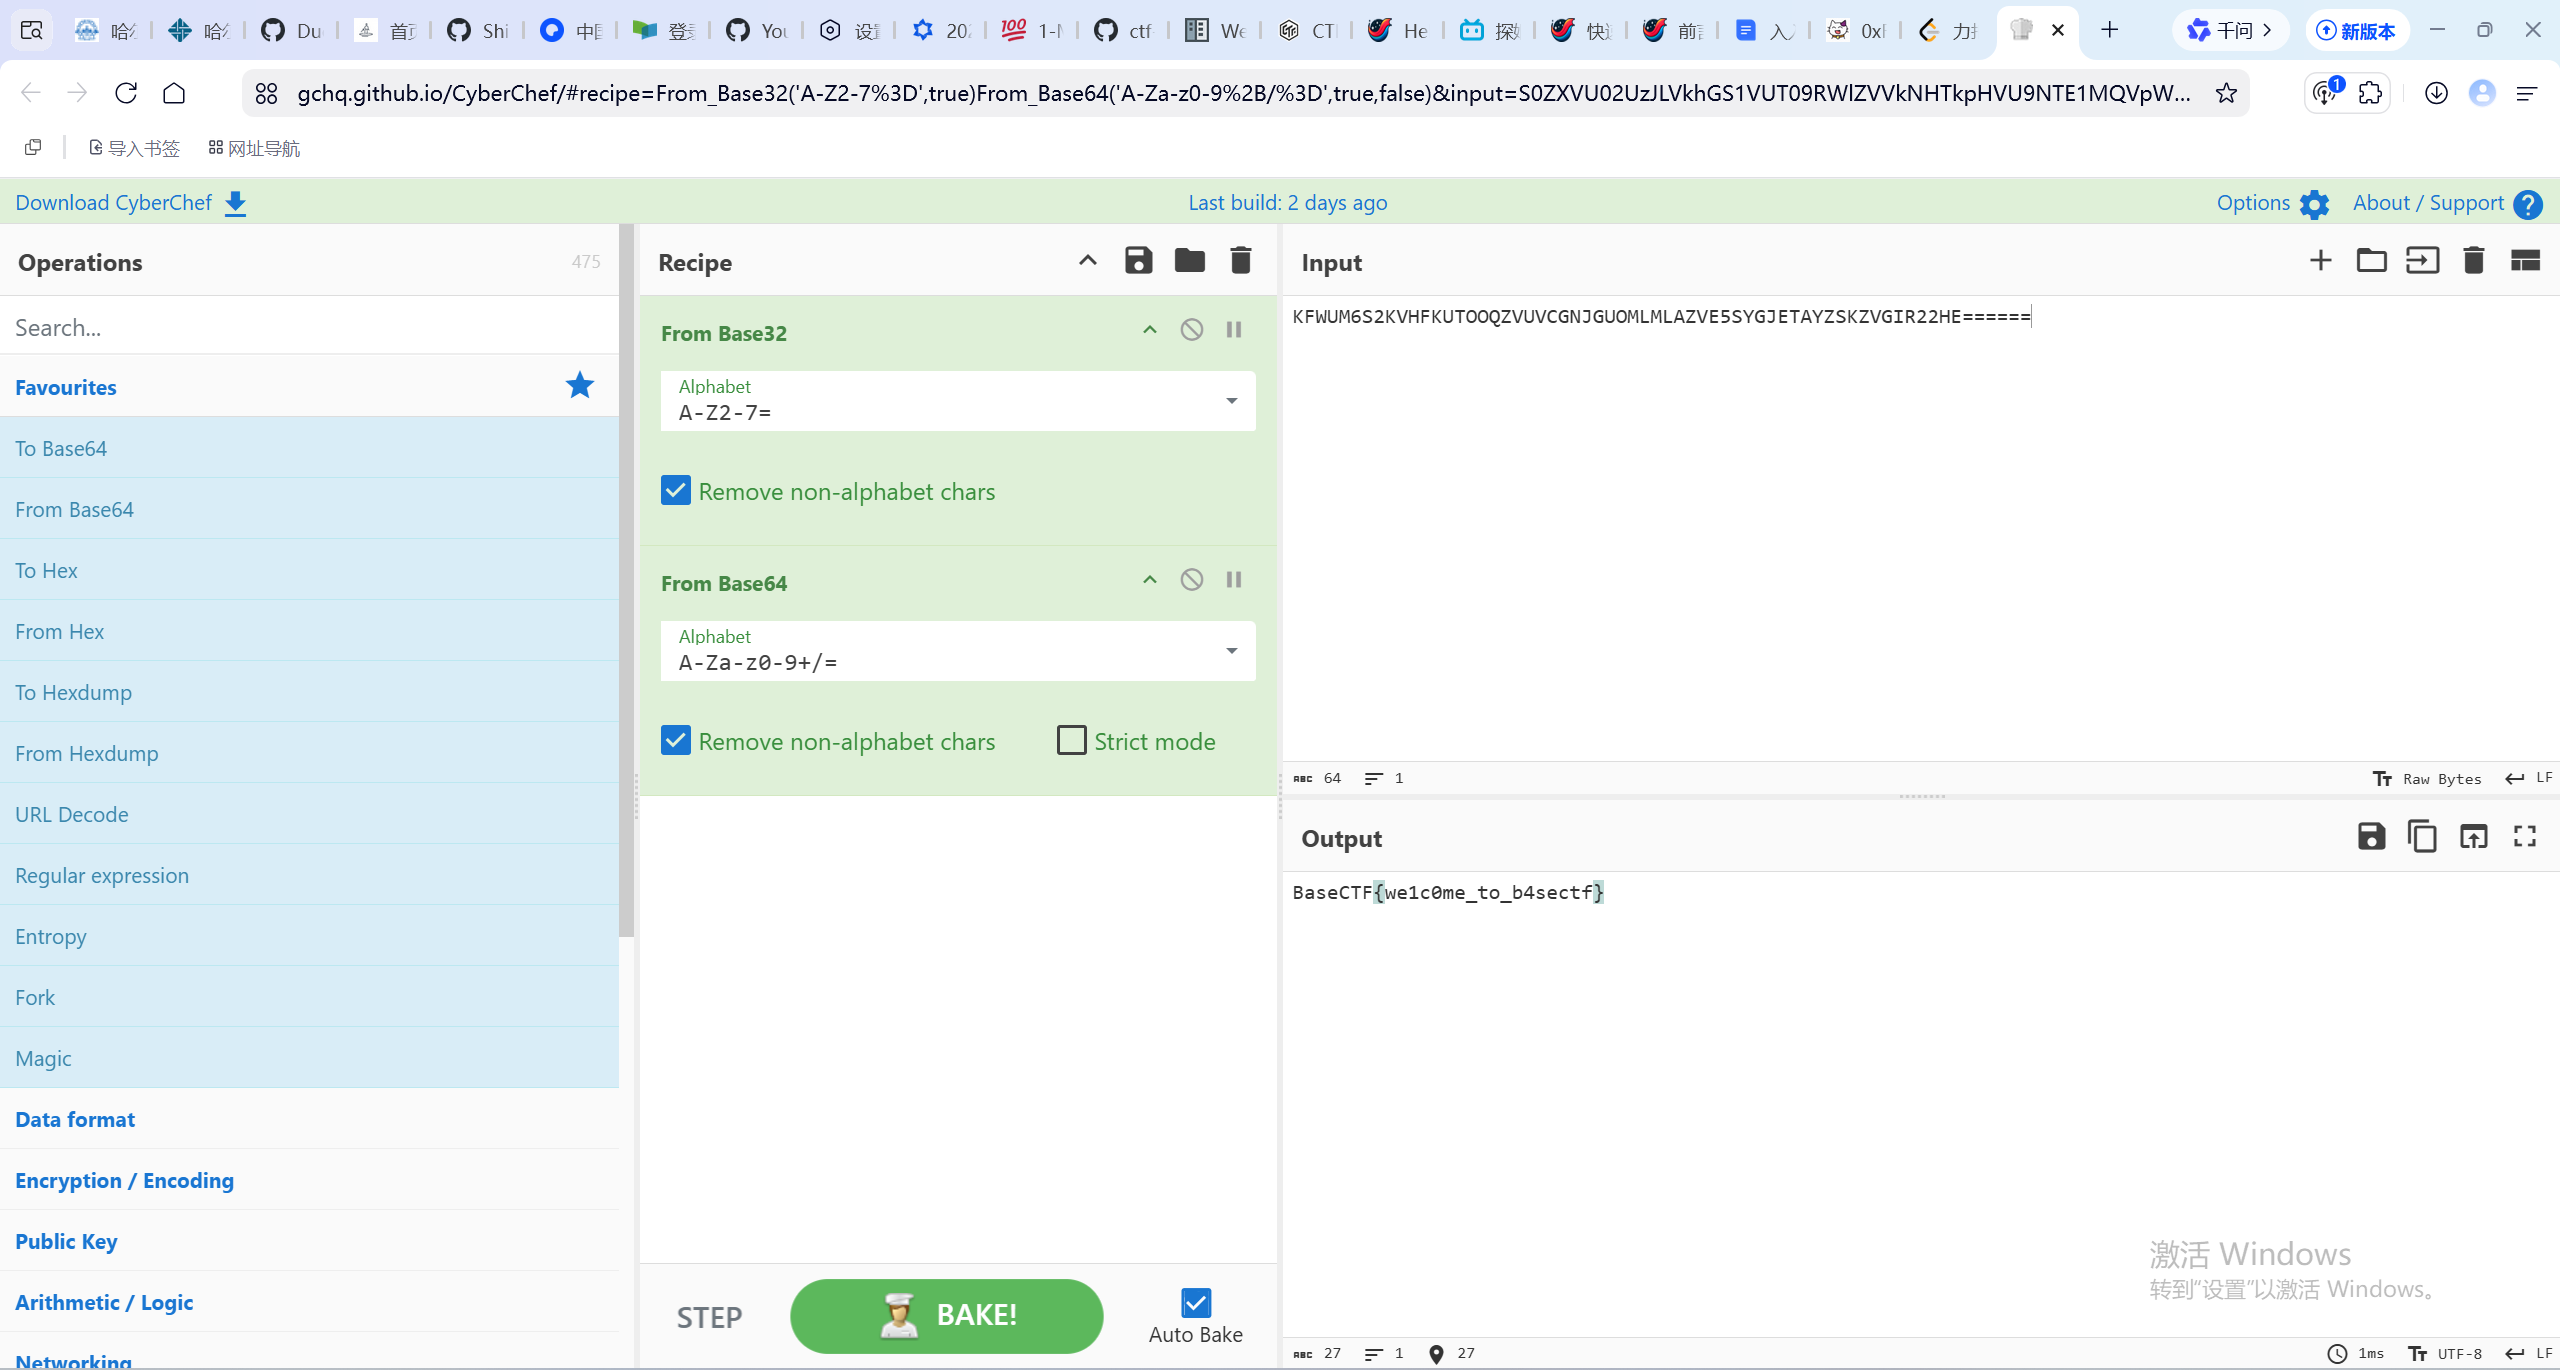
\includegraphics[width=0.95\textwidth]{1.png}
    \caption{CyberChef 双层解码界面}
\end{figure}

\subsection{最终Flag}
\begin{center}
    \Large flag\{we1c0me\_to\_b4sectf\}
\end{center}

\newpage

% --------------------- 题目2：PyJail Truncate 截断绕过
\section{题目2：PyJail Truncate 截断绕过}
\subsection{题目分析}
该题目为一个 Python 沙箱（PyJail）程序，核心代码如下：
\begin{verbatim}
flag = open("flag.txt", "r").read().strip()
eval(input("输入: ")[:8])
\end{verbatim}
限制：用户输入会被截断为前 8 个字符，然后传入 eval() 执行。目标是在 8 个字符内泄露 flag 变量的值。

\subsection{解题步骤}
\begin{enumerate}
    \item 直接使用 (flag) 输出变量值，但长度为 6 个字符，理论上可行，但无法直接打印。
    \item 利用 Python eval() 的 NFKC 规范化特性，使用 Unicode 连字字符 fl（U+FB02），它会被自动规范化为 fl。
    \item 构造 Payload int(flag)，长度为 7 个字符，满足截断限制。执行时 int(flag) 会因 flag 为字符串而报错，但错误信息中会泄露 flag 的完整内容。
    \item 使用 nc 连接到靶机，输入 Payload 即可从报错信息中获取 flag。
\end{enumerate}

\begin{figure}[H]
    \centering
    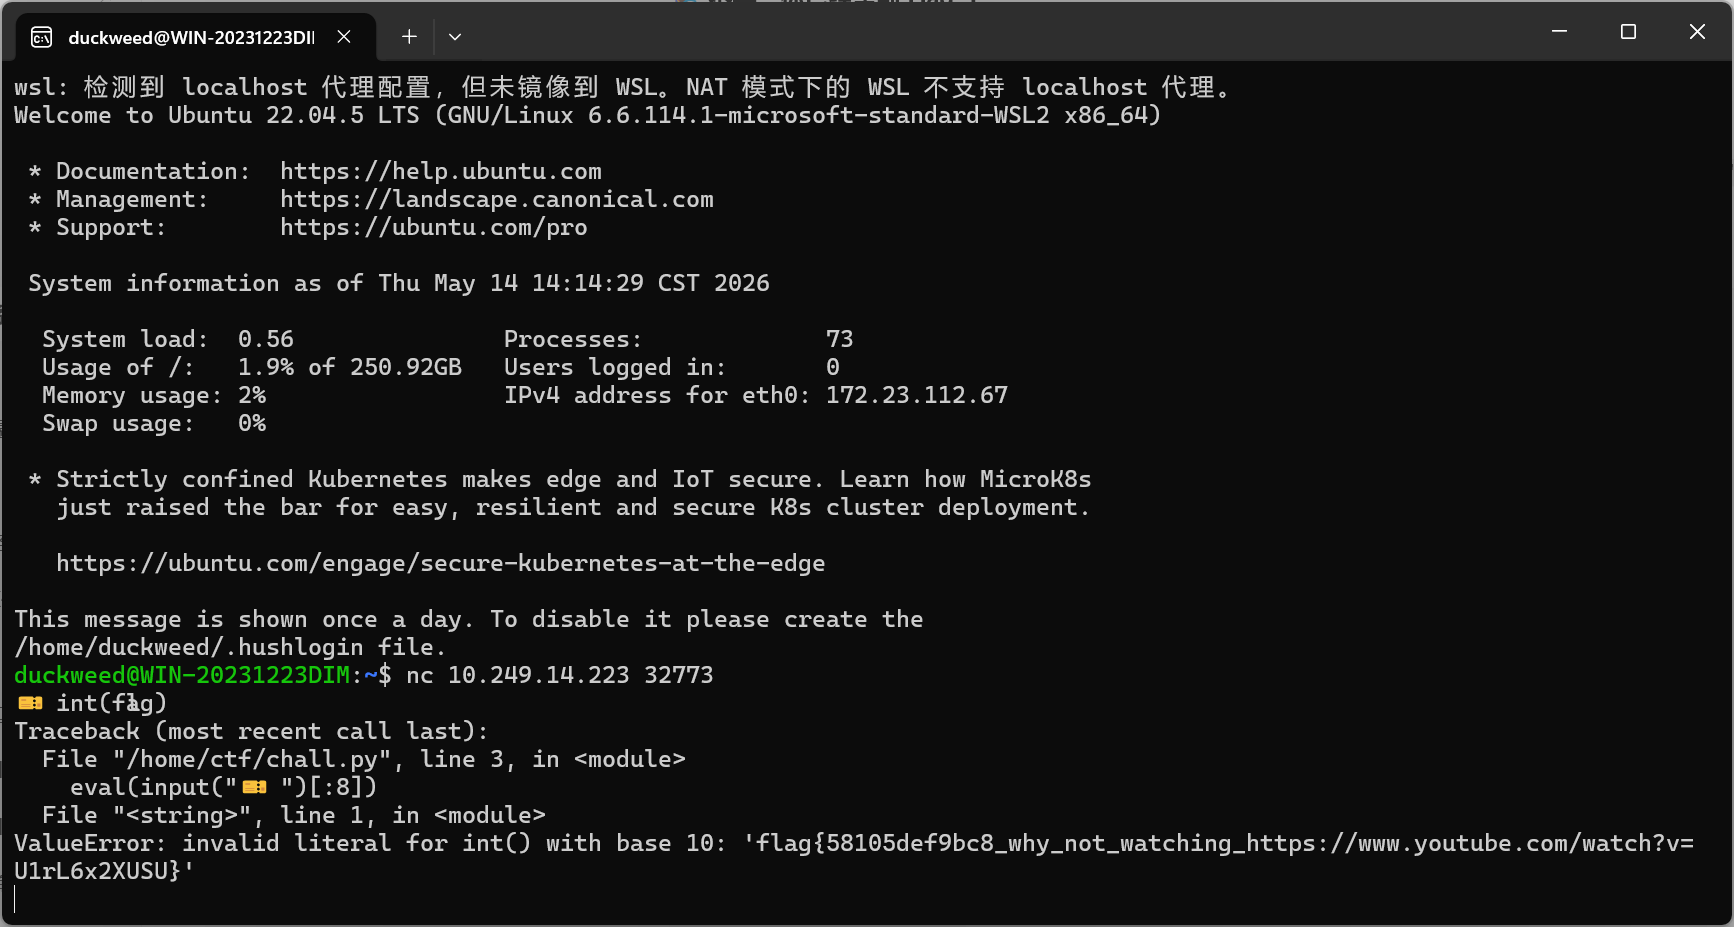
\includegraphics[width=0.95\textwidth]{2.1.png}
    \caption{nc 连接靶机并获取 flag}
\end{figure}

\subsection{最终Flag}
\begin{center}
    \Large flag\{58105def9bc8\_why\_not\_watching\_https://www.youtube.com/watch?v=U1rL6x2XUSU\}
\end{center}

\newpage

% --------------------- 题目3
\section{题目3：图像隐写LSB}
\subsection{解题步骤}
\begin{enumerate}
    \item 使用 010 Editor 查看文件头，确认文件类型为 PNG。
    \item 使用 StegSolve 工具提取图片最低有效位（LSB）数据。
    \item 从提取数据中得到 flag。
\end{enumerate}

\begin{figure}[H]
    \centering
    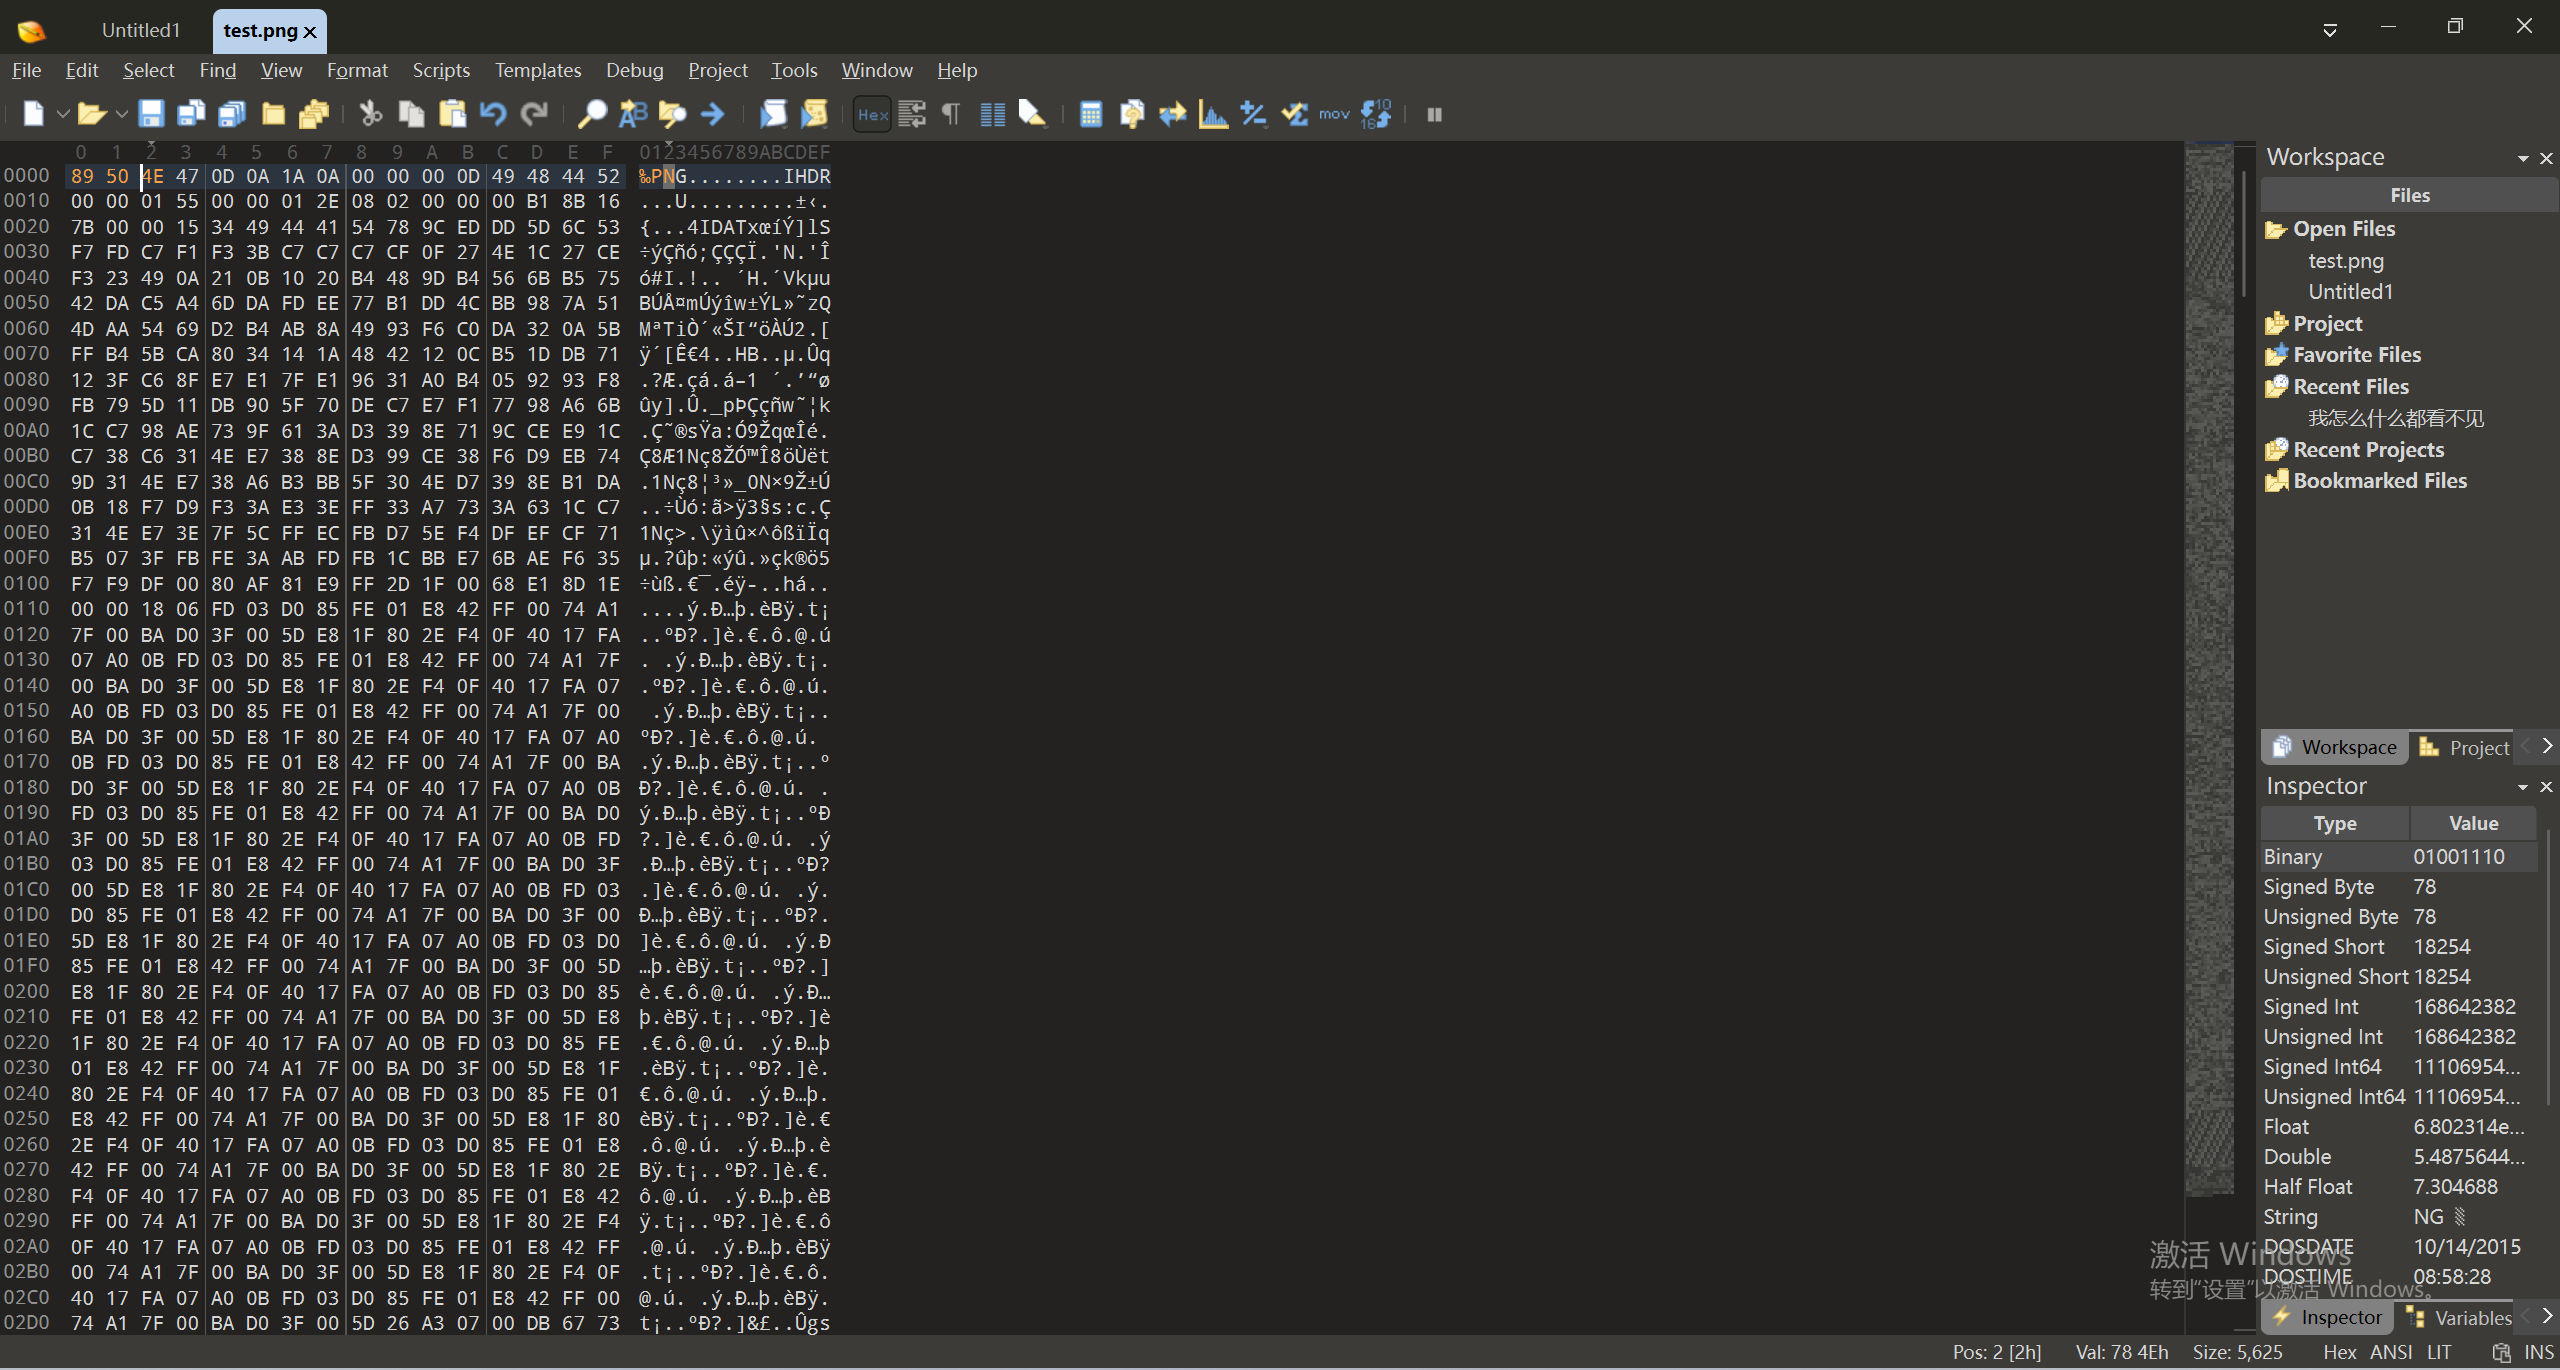
\includegraphics[width=0.95\textwidth]{3.1.png}
    \caption{010 Editor 查看文件头}
\end{figure}
\begin{figure}[H]
    \centering
    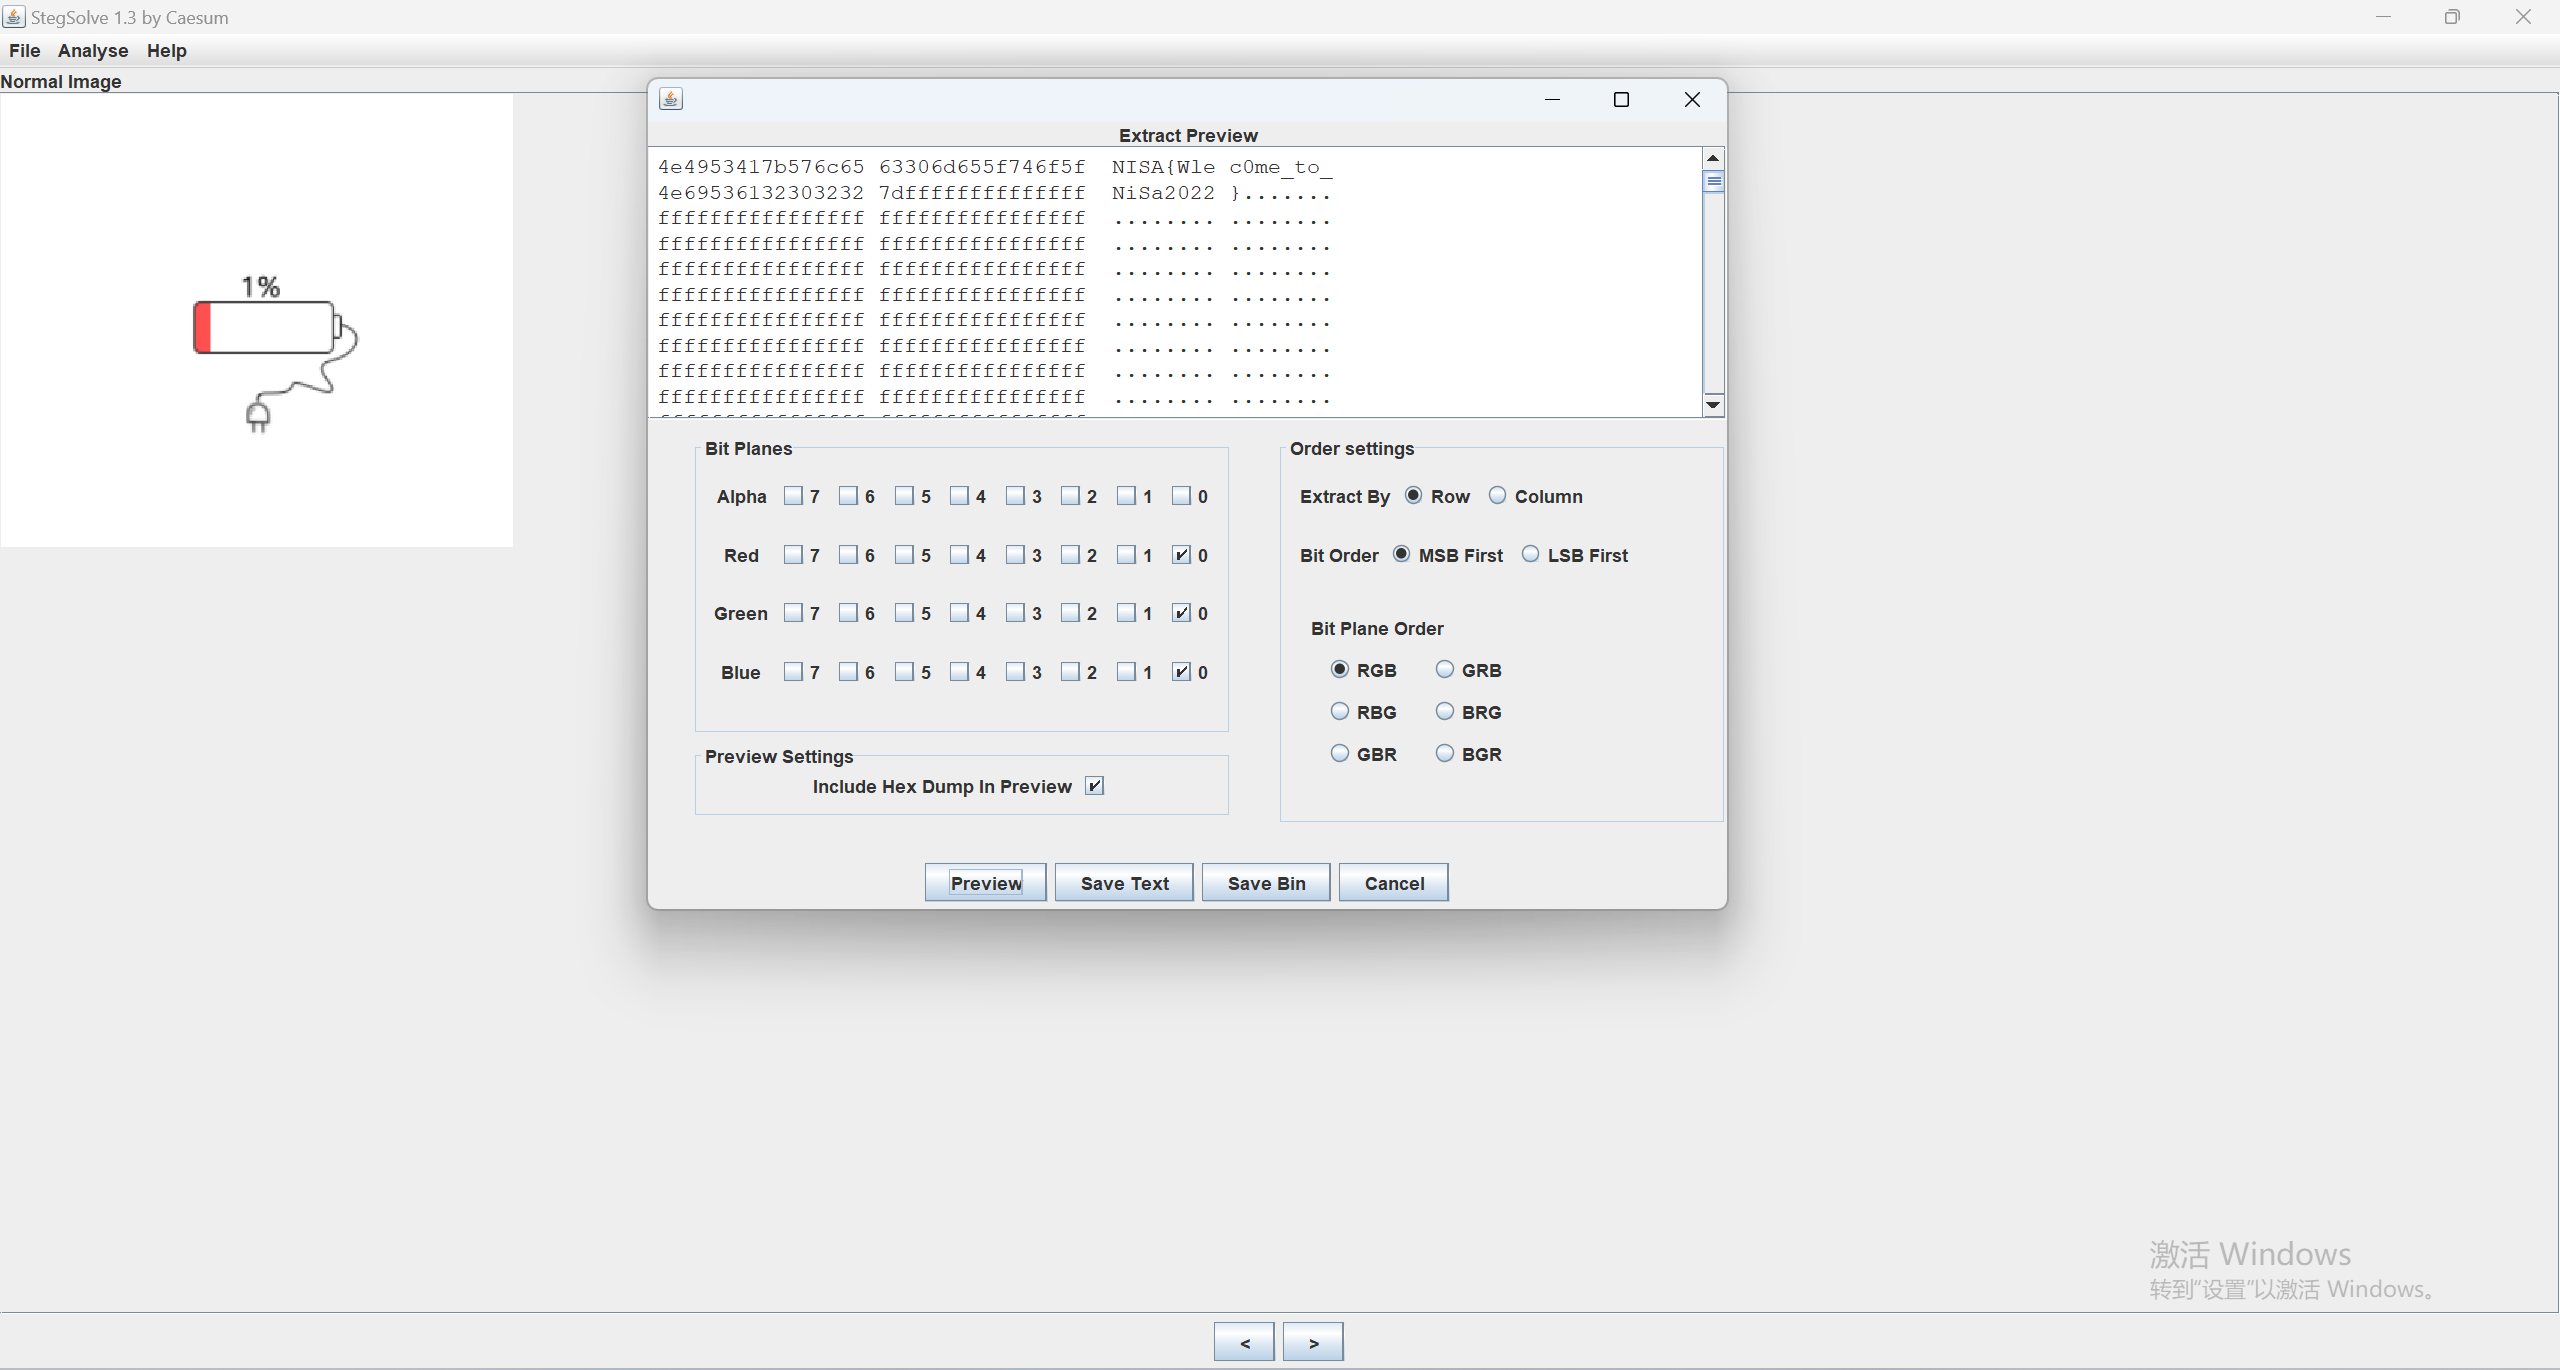
\includegraphics[width=0.95\textwidth]{3.2.png}
    \caption{StegSolve 提取 LSB 数据}
\end{figure}

\subsection{最终Flag}
\begin{center}
    \Large NISA\{Wlec0me\_to\_NiSa2022\}
\end{center}

\newpage

% --------------------- 题目4：音频隐写
\section{题目4：音频隐写（摩斯密码）}
\subsection{解题步骤}
\begin{enumerate}
    \item 使用 Audacity 打开音频文件，观察波形识别摩斯密码。
    \item 将识别到的摩斯密码进行解码，得到明文 flag。
\end{enumerate}

\begin{figure}[H]
    \centering
    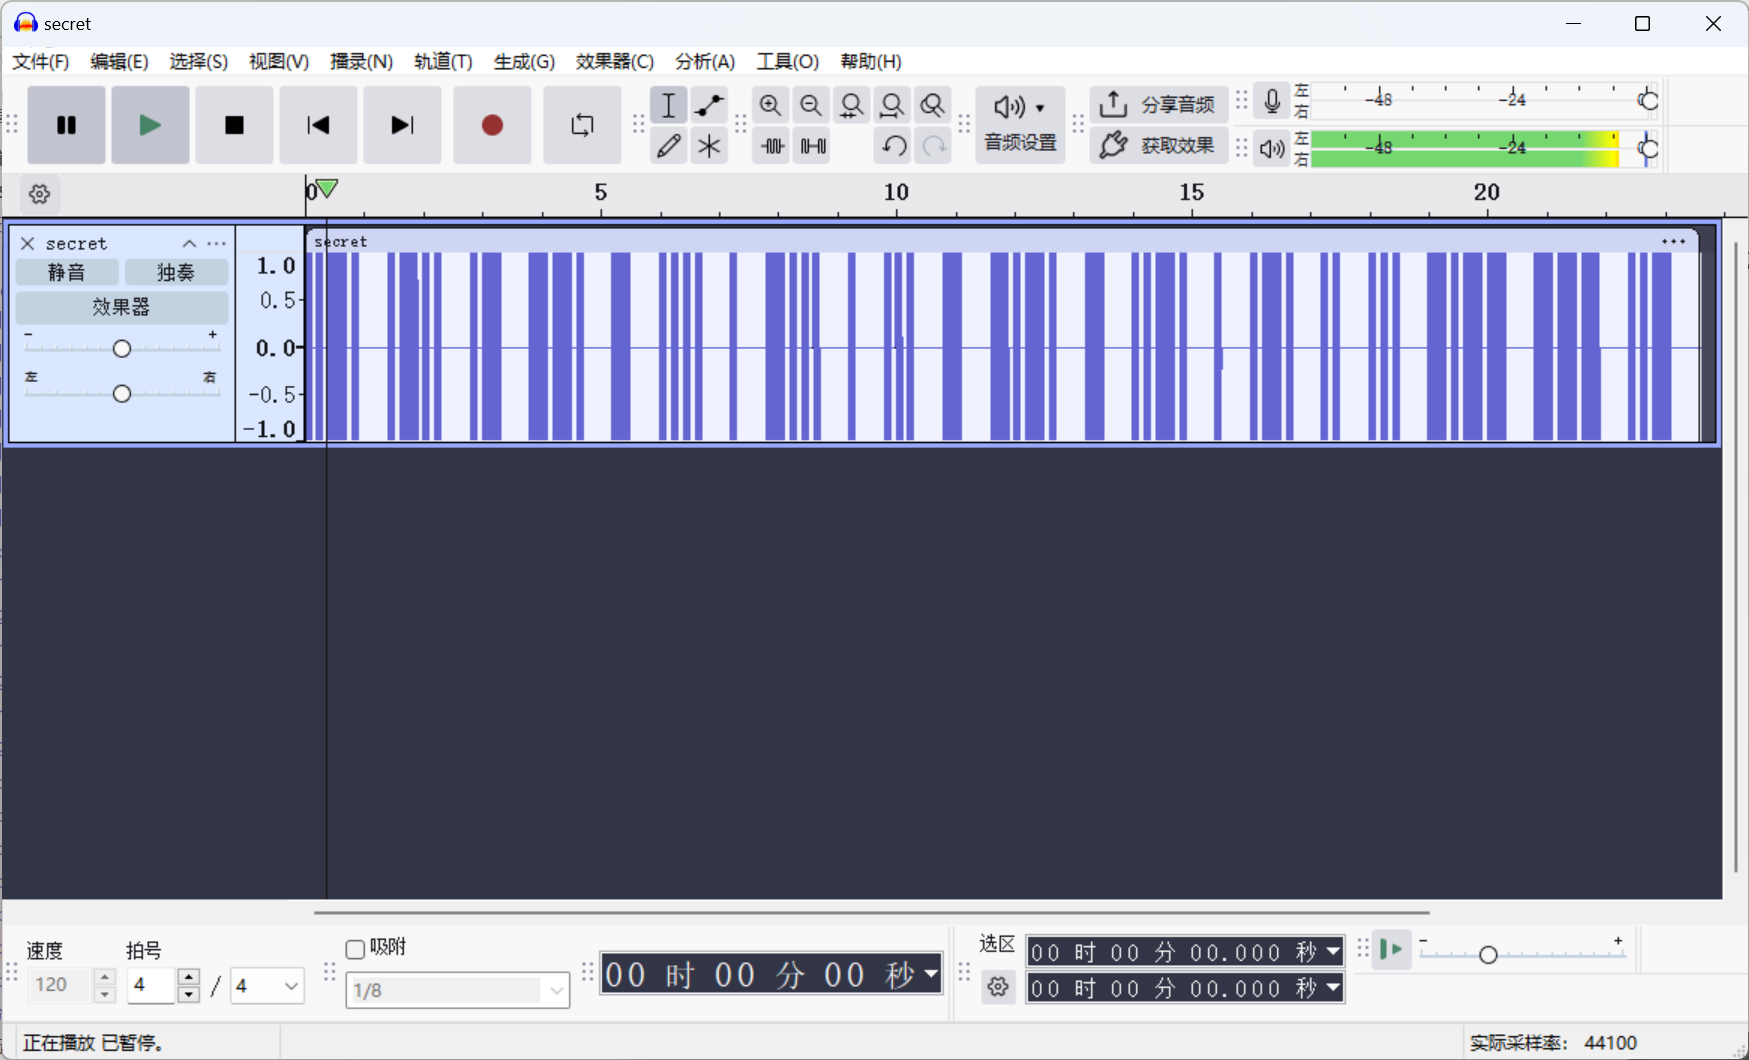
\includegraphics[width=0.95\textwidth]{4.1.png}
    \caption{Audacity 音频波形图}
\end{figure}
\begin{figure}[H]
    \centering
    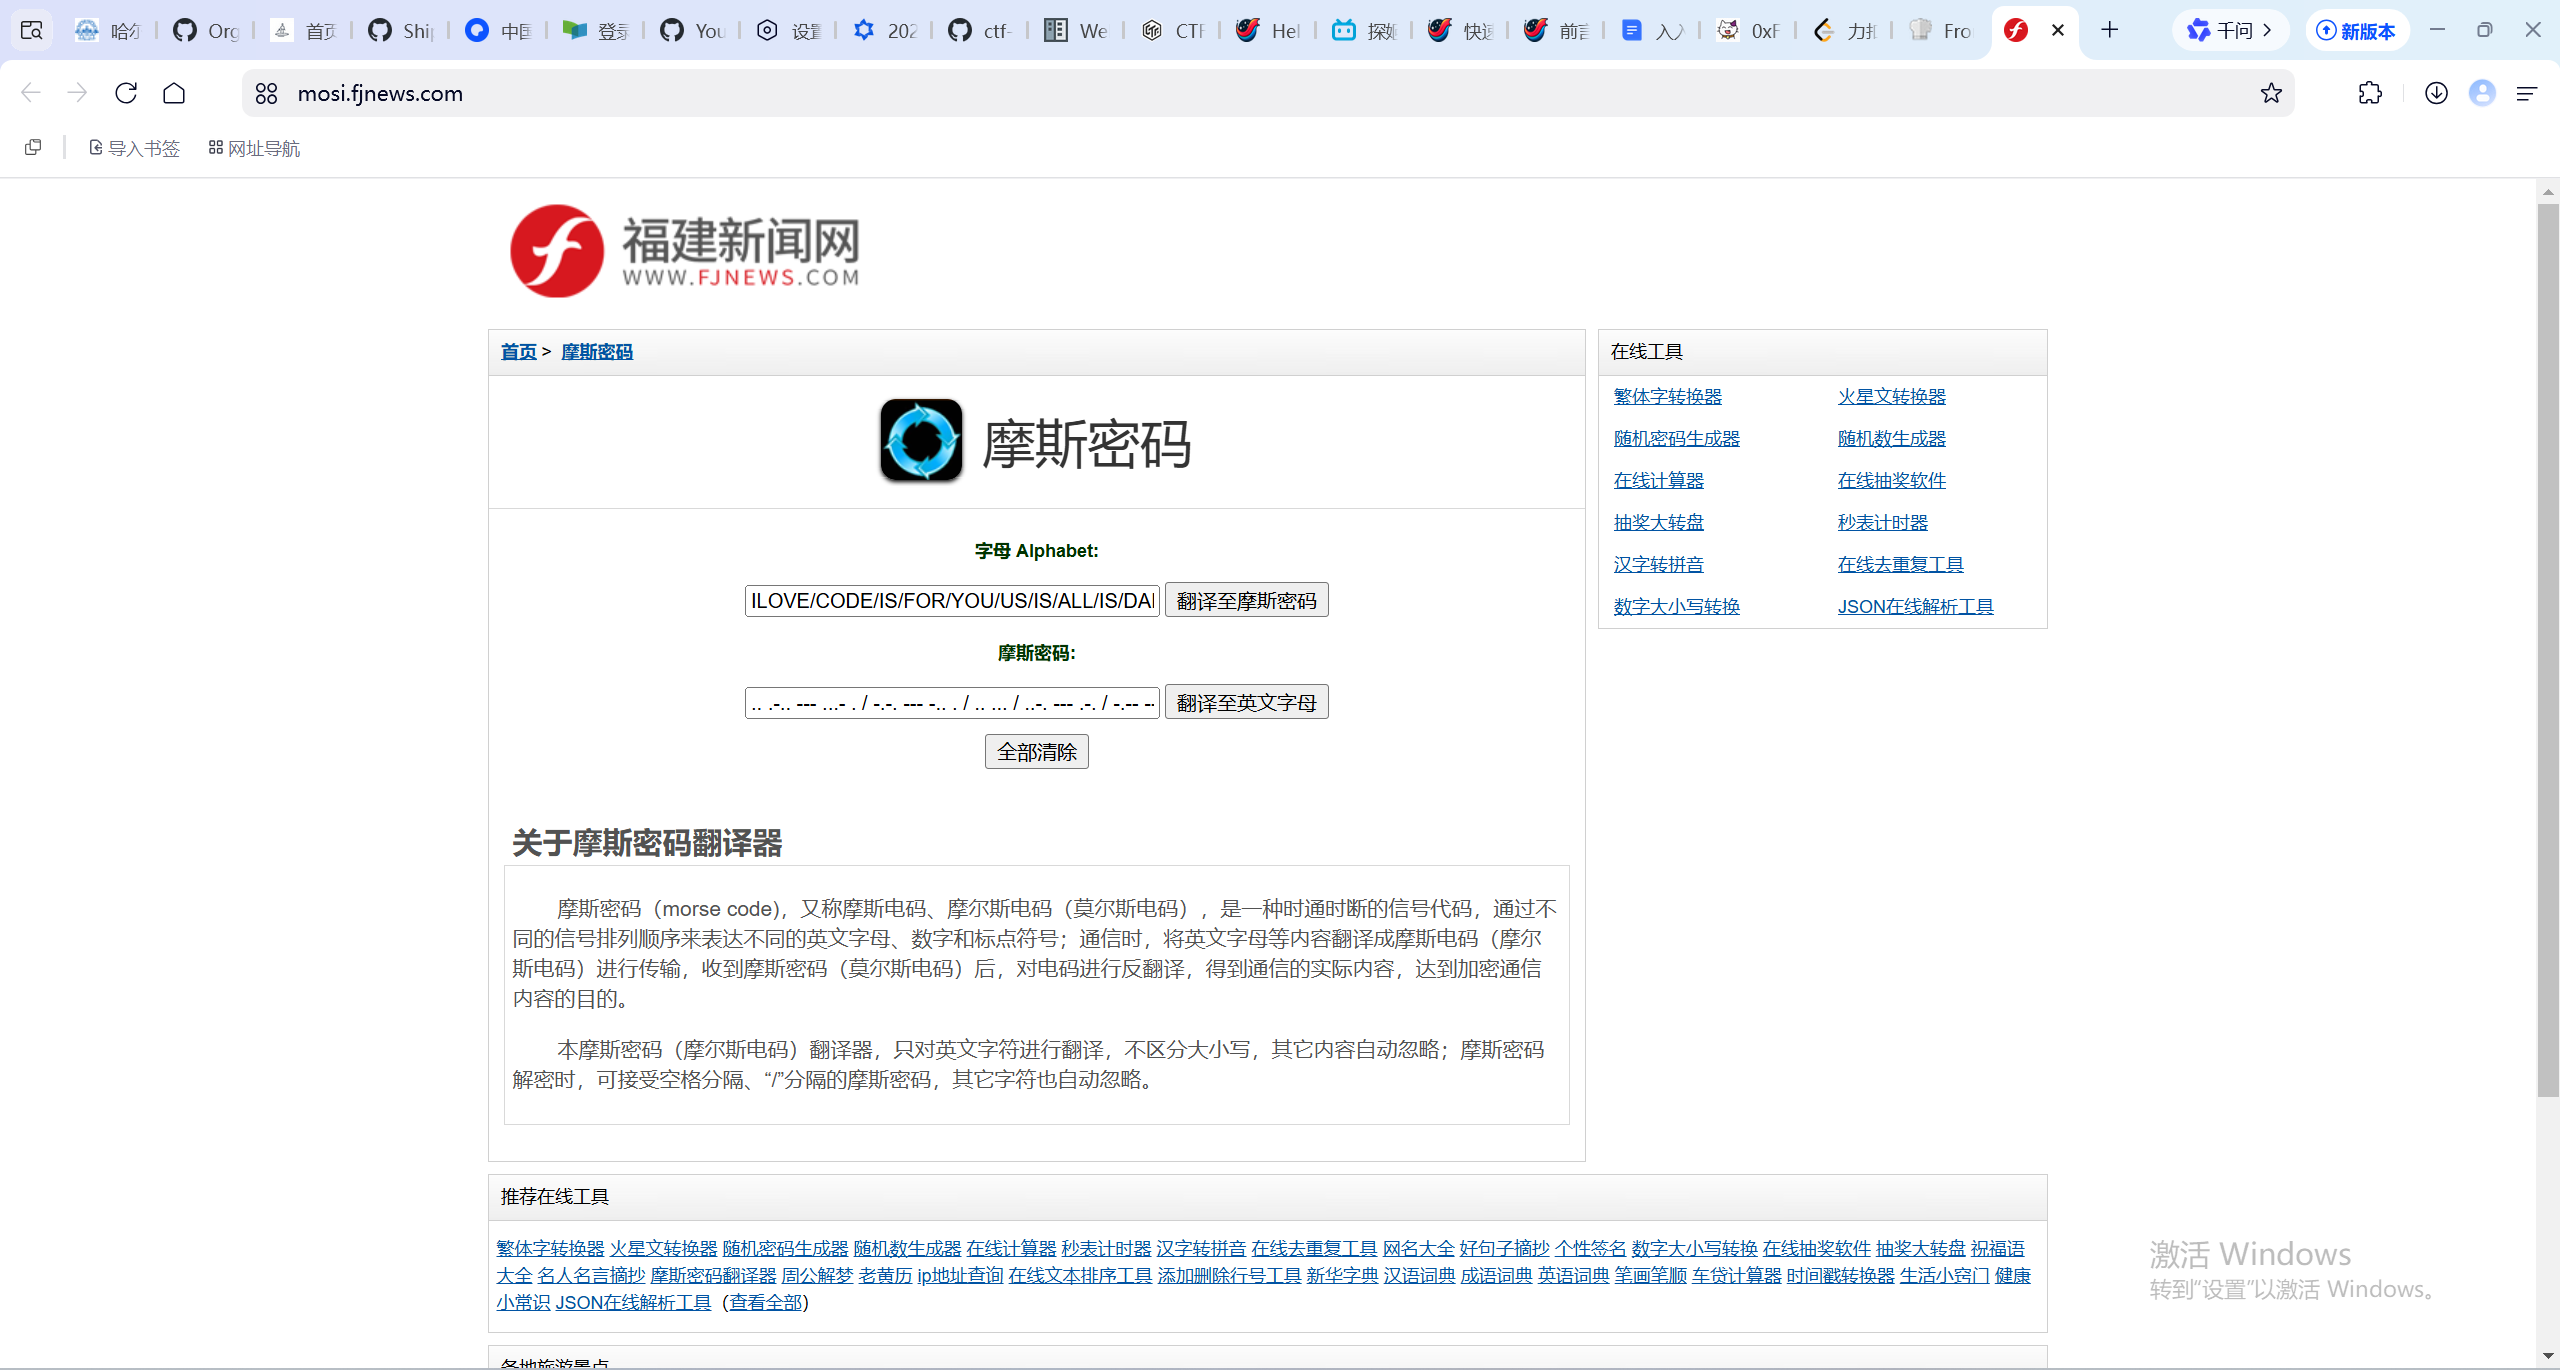
\includegraphics[width=0.95\textwidth]{4.2.png}
    \caption{摩斯密码解码结果}
\end{figure}

\subsection{最终Flag}
\begin{center}
    \Large flag\{thebestctferisyou\}
\end{center}

\newpage

% --------------------- 题目5：文本隐写（零宽字符 · 330k 官方工具）
\section{题目5：文本隐写（Unicode 零宽字符隐写）}
\subsection{解题步骤}
\begin{enumerate}
    \item 打开 330k 官方零宽字符隐写工具：\url{http://330k.github.io/misc_tools/unicode_steganography.html}
    \item 将含隐写的文本粘贴到工具中，点击 Decode 进行解密。
    \item 工具自动提取隐藏在 Unicode 零宽字符中的信息，得到最终 flag。
\end{enumerate}

\begin{figure}[H]
    \centering
    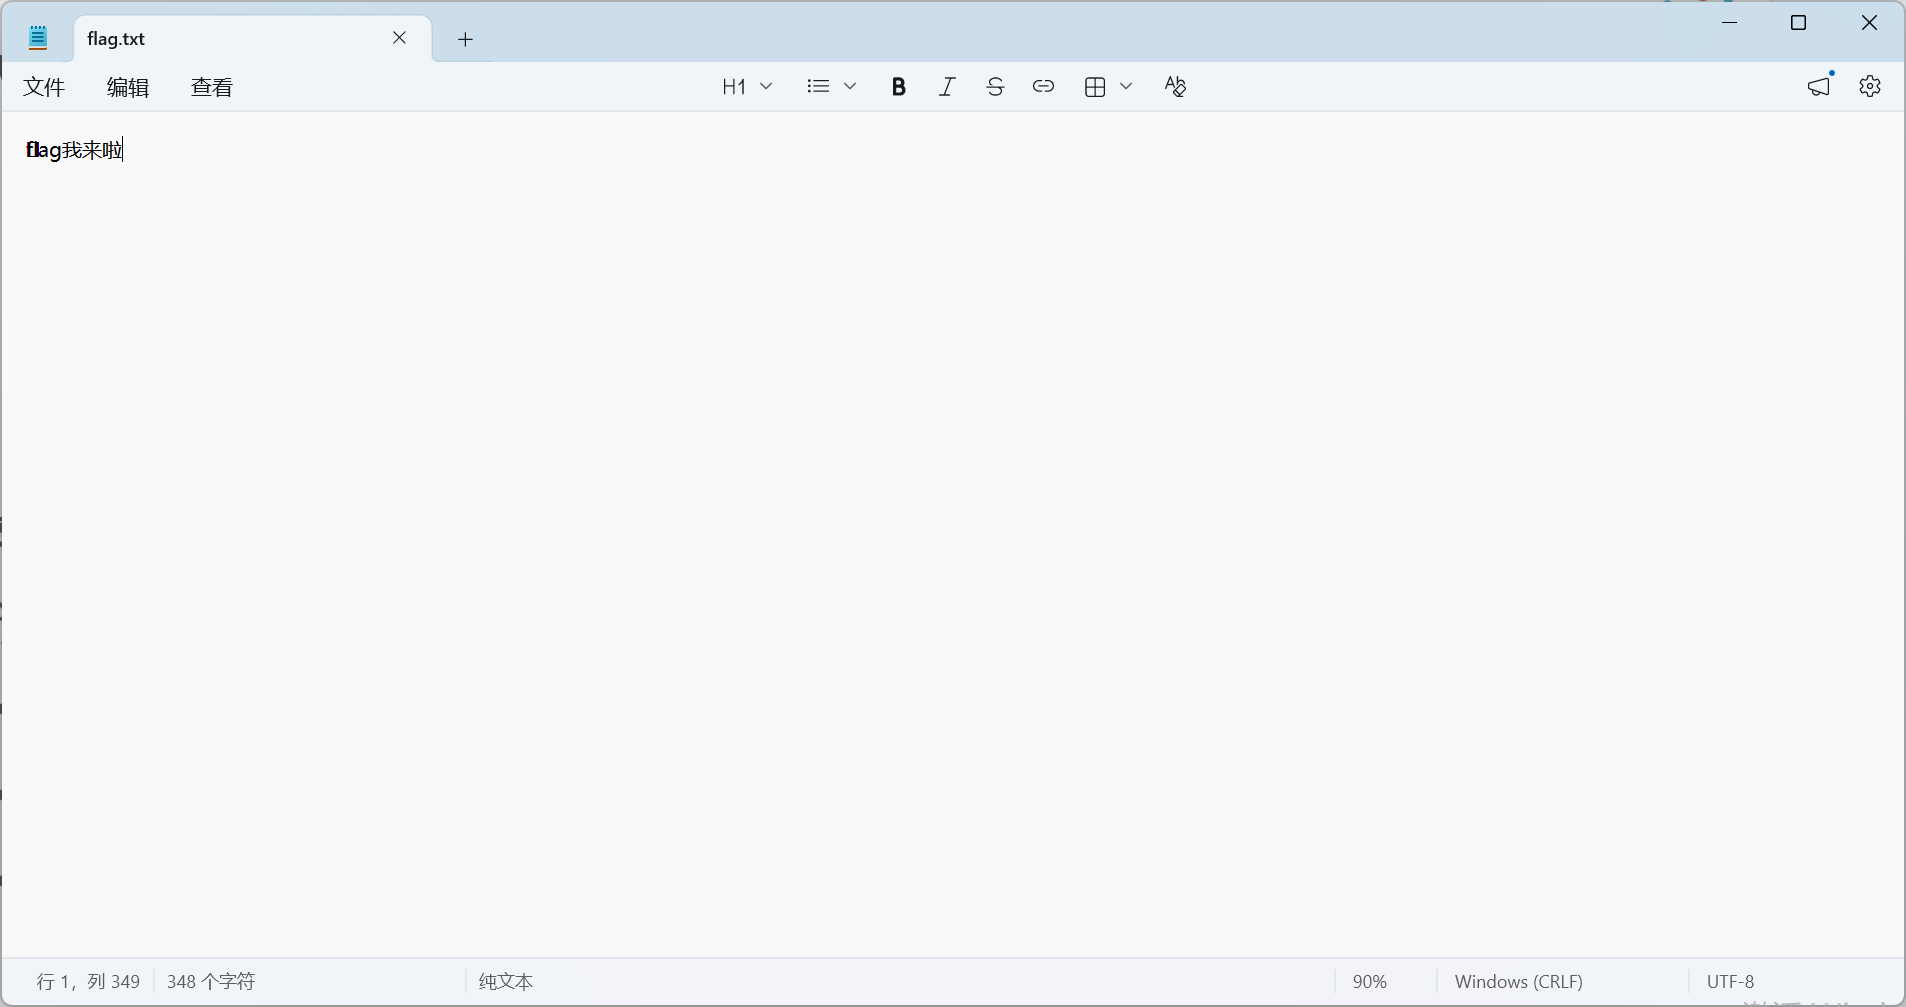
\includegraphics[width=0.95\textwidth]{5.1.png}
    \caption{零宽隐写文本内容查看}
\end{figure}
\begin{figure}[H]
    \centering
    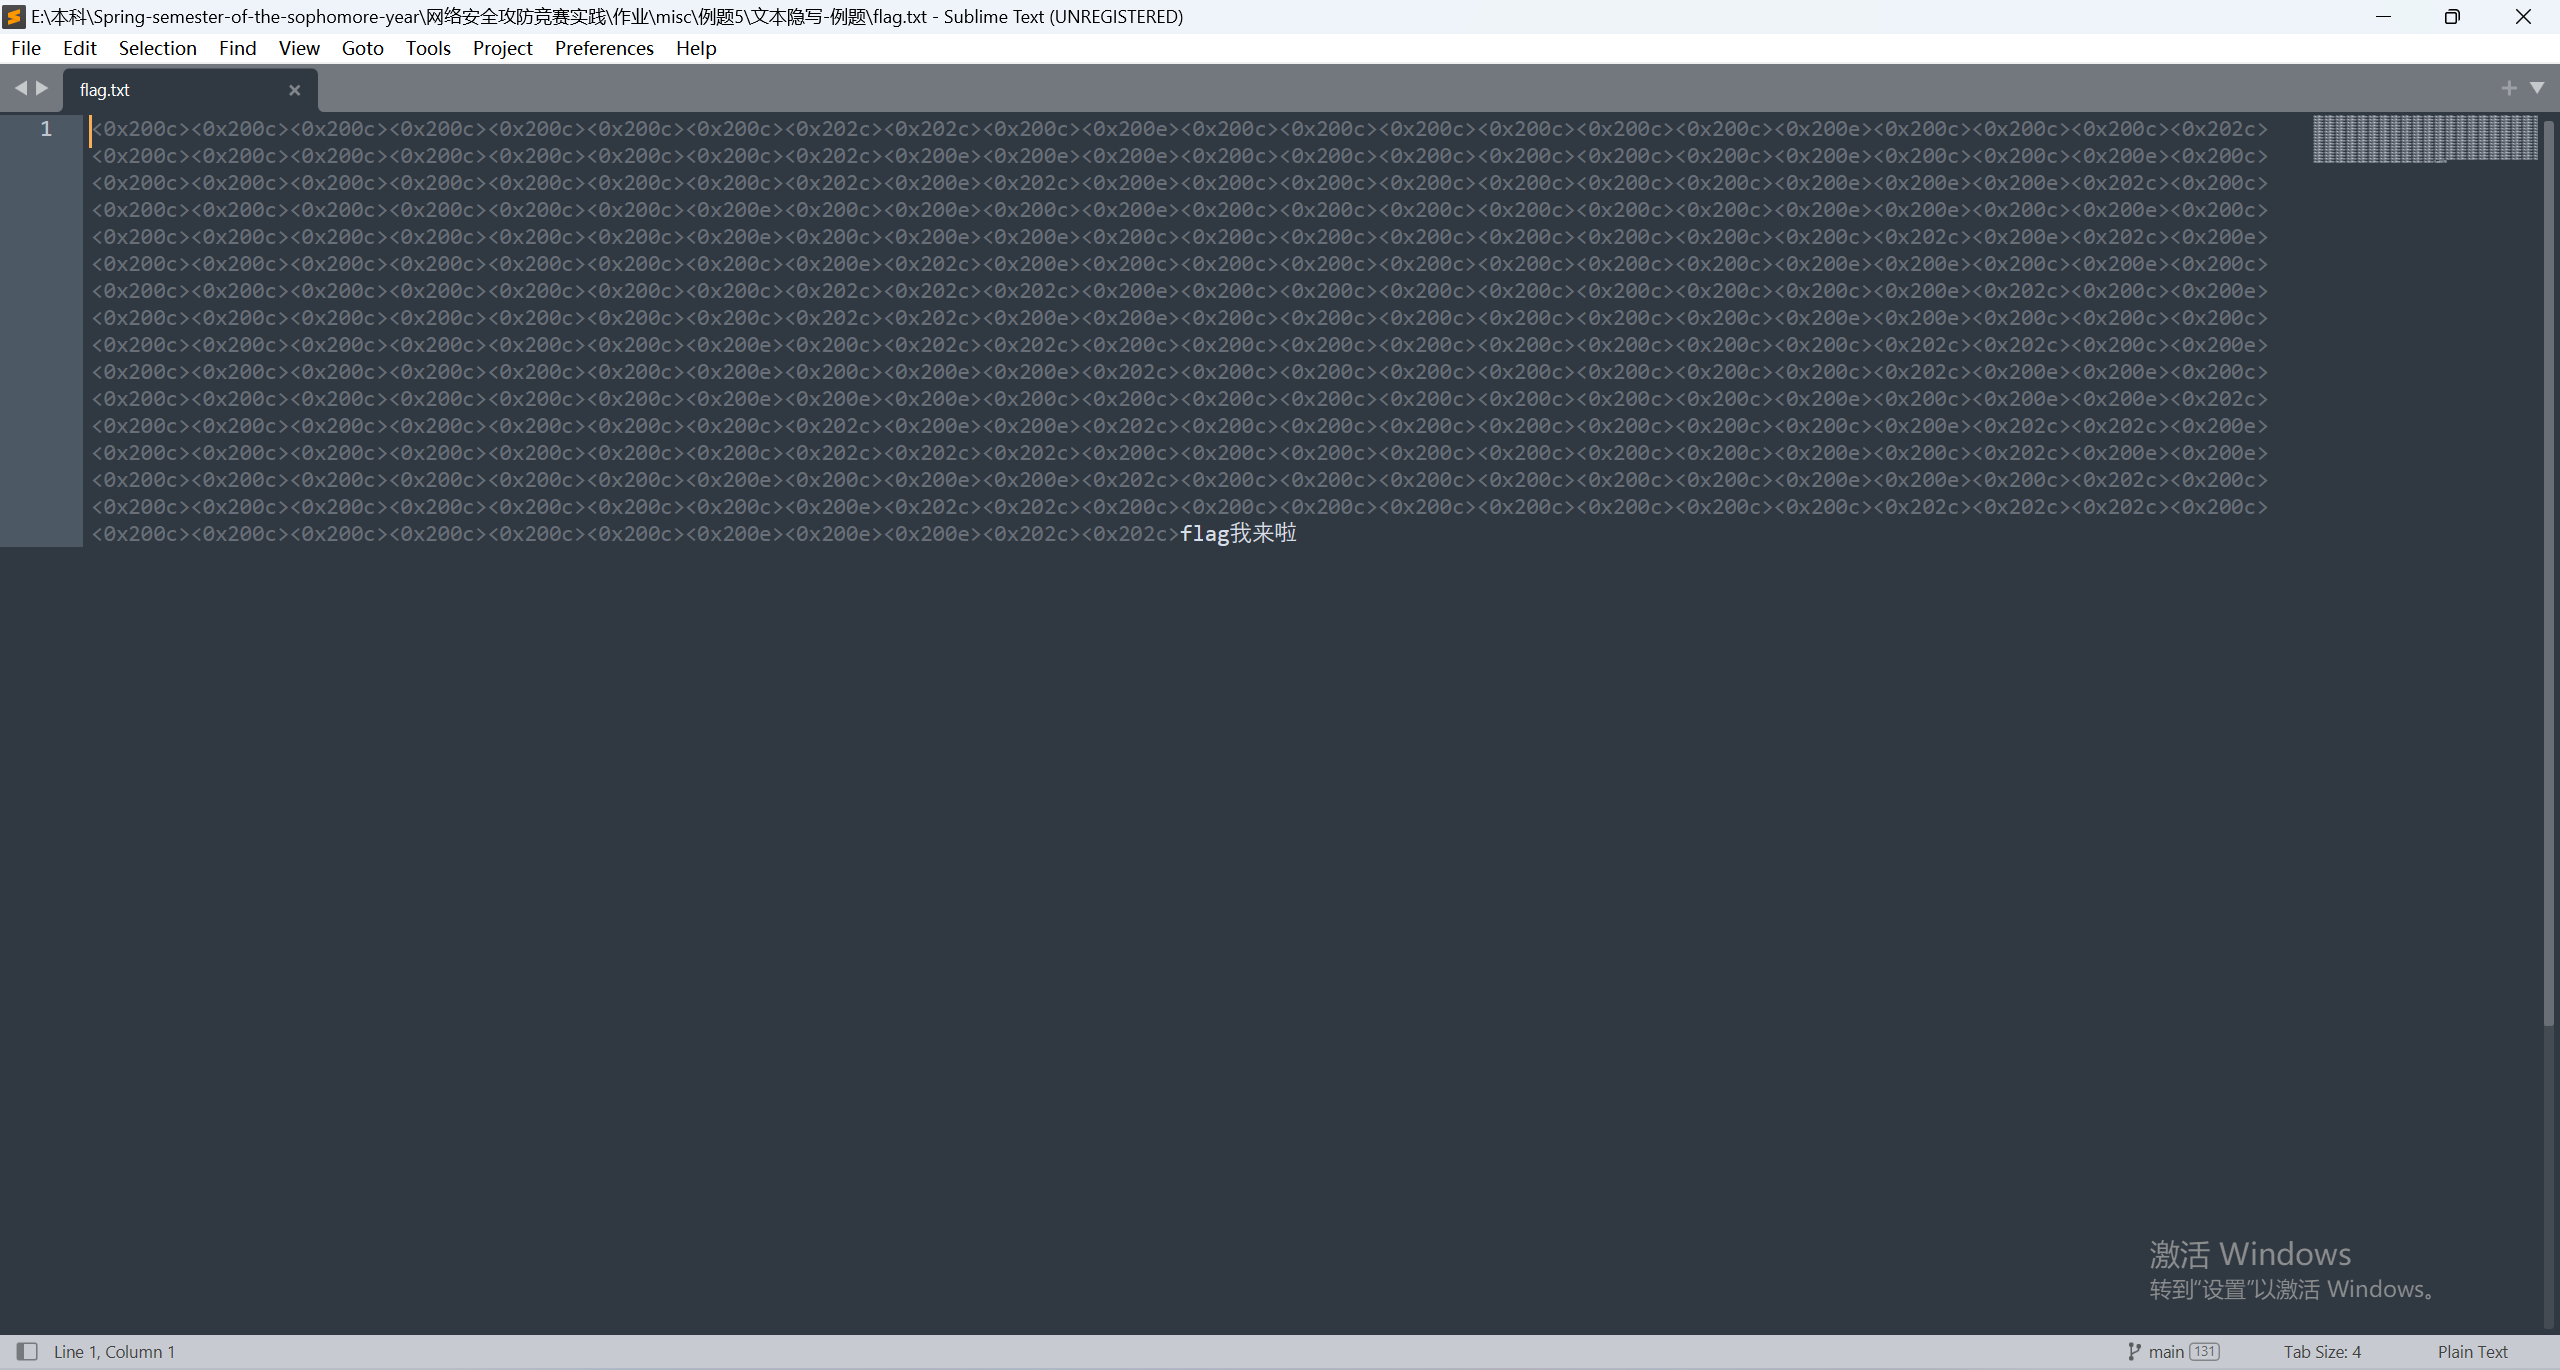
\includegraphics[width=0.95\textwidth]{5.2.png}
    \caption{330k 零宽隐写工具解密界面}
\end{figure}
\begin{figure}[H]
    \centering
    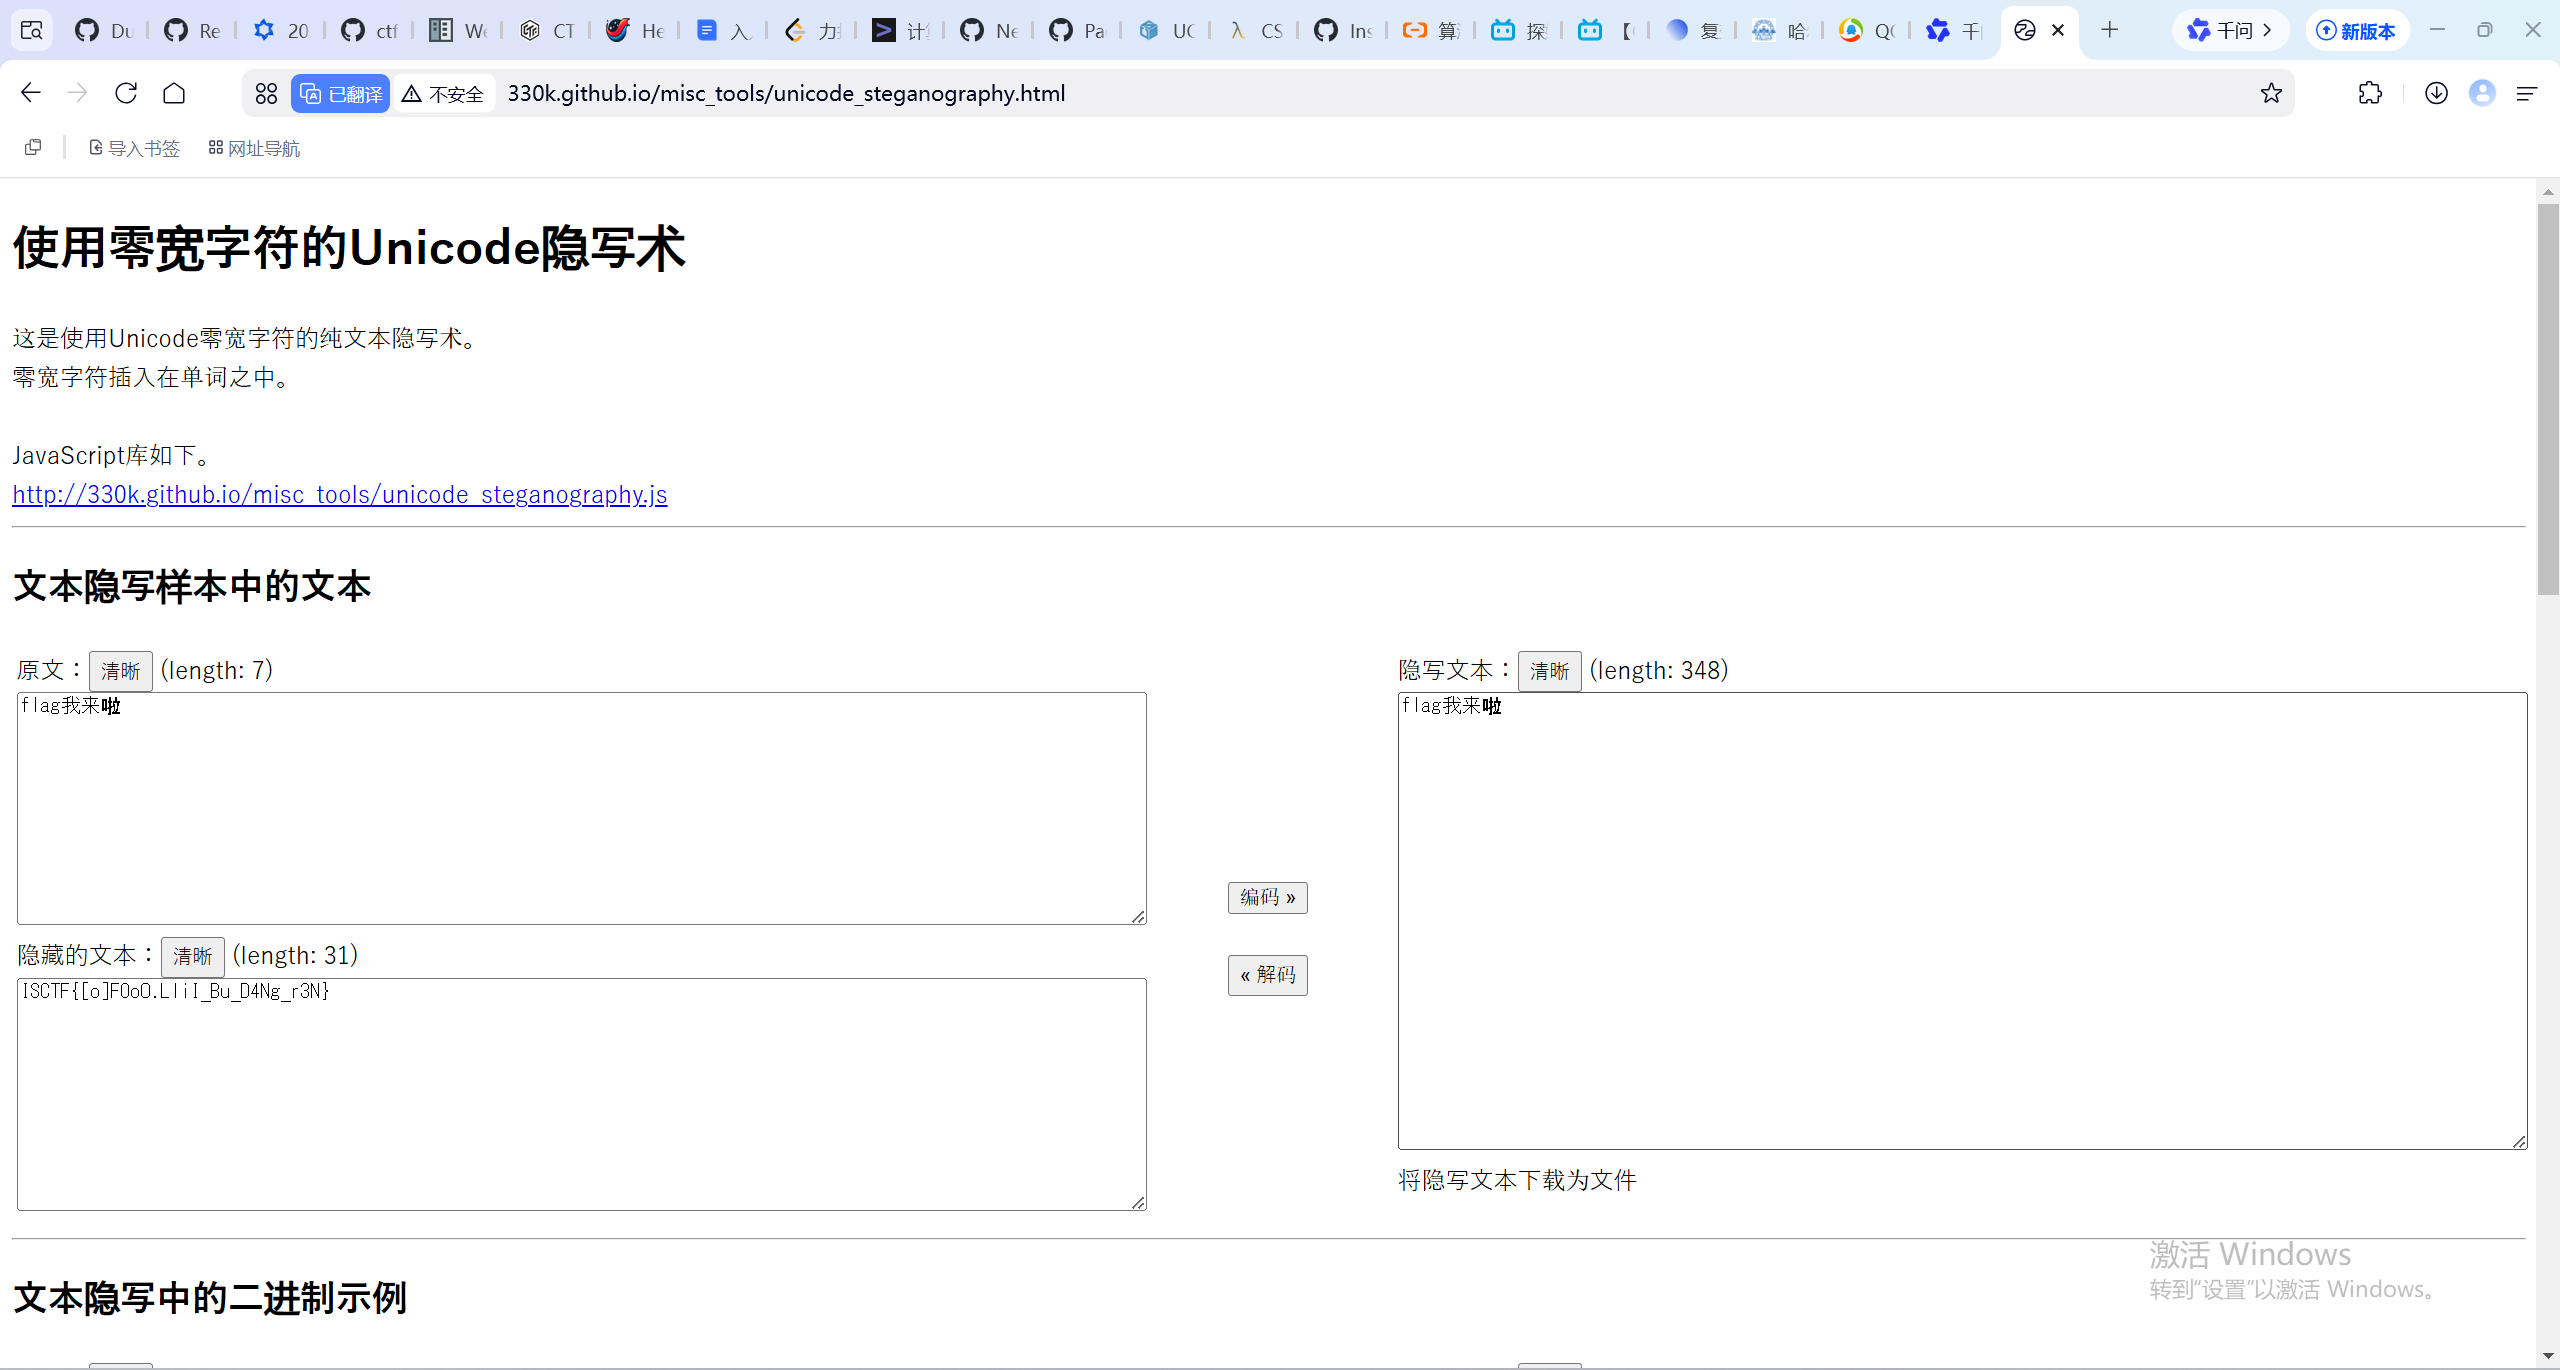
\includegraphics[width=0.95\textwidth]{5.3.png}
    \caption{工具解密得到隐藏 flag}
\end{figure}

\subsection{最终Flag}
\begin{center}
    \Large ISCTF\{[o]F0oO.LliI\_Bu\_D4Ng\_r3N\}
\end{center}

\newpage

% --------------------- 题目6：ZIP爆破 + Steghide图像隐写
\section{题目6：ZIP爆破 + Steghide图像隐写}
\subsection{题目分析}
该题目为典型的多步骤隐写题，需要先爆破加密ZIP包，再通过Base64解码获取隐写密码，最后使用Steghide工具从图片中提取隐藏的flag。

\subsection{解题步骤}
\begin{enumerate}
    \item 使用ARCHPR工具暴力破解加密的ez隐写.zip，得到解压密码ctf。
    \item 解压得到hint.txt和haibara.jpg，hint.txt中为Base64编码的字符串。
    \item 使用CyberChef对Base64字符串解码，得到隐写密码welcome\_to\_my\_world。
    \item 在WSL中使用steghide工具，通过解码得到的密码从haibara.jpg中提取隐藏文件。
    \item 提取成功后，得到flag.txt，即为最终flag。
\end{enumerate}

\begin{figure}[H]
    \centering
    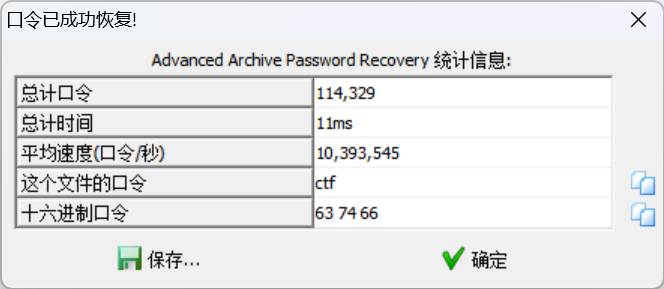
\includegraphics[width=0.95\textwidth]{6.1.png}
    \caption{ARCHPR爆破得到ZIP密码}
\end{figure}
\begin{figure}[H]
    \centering
    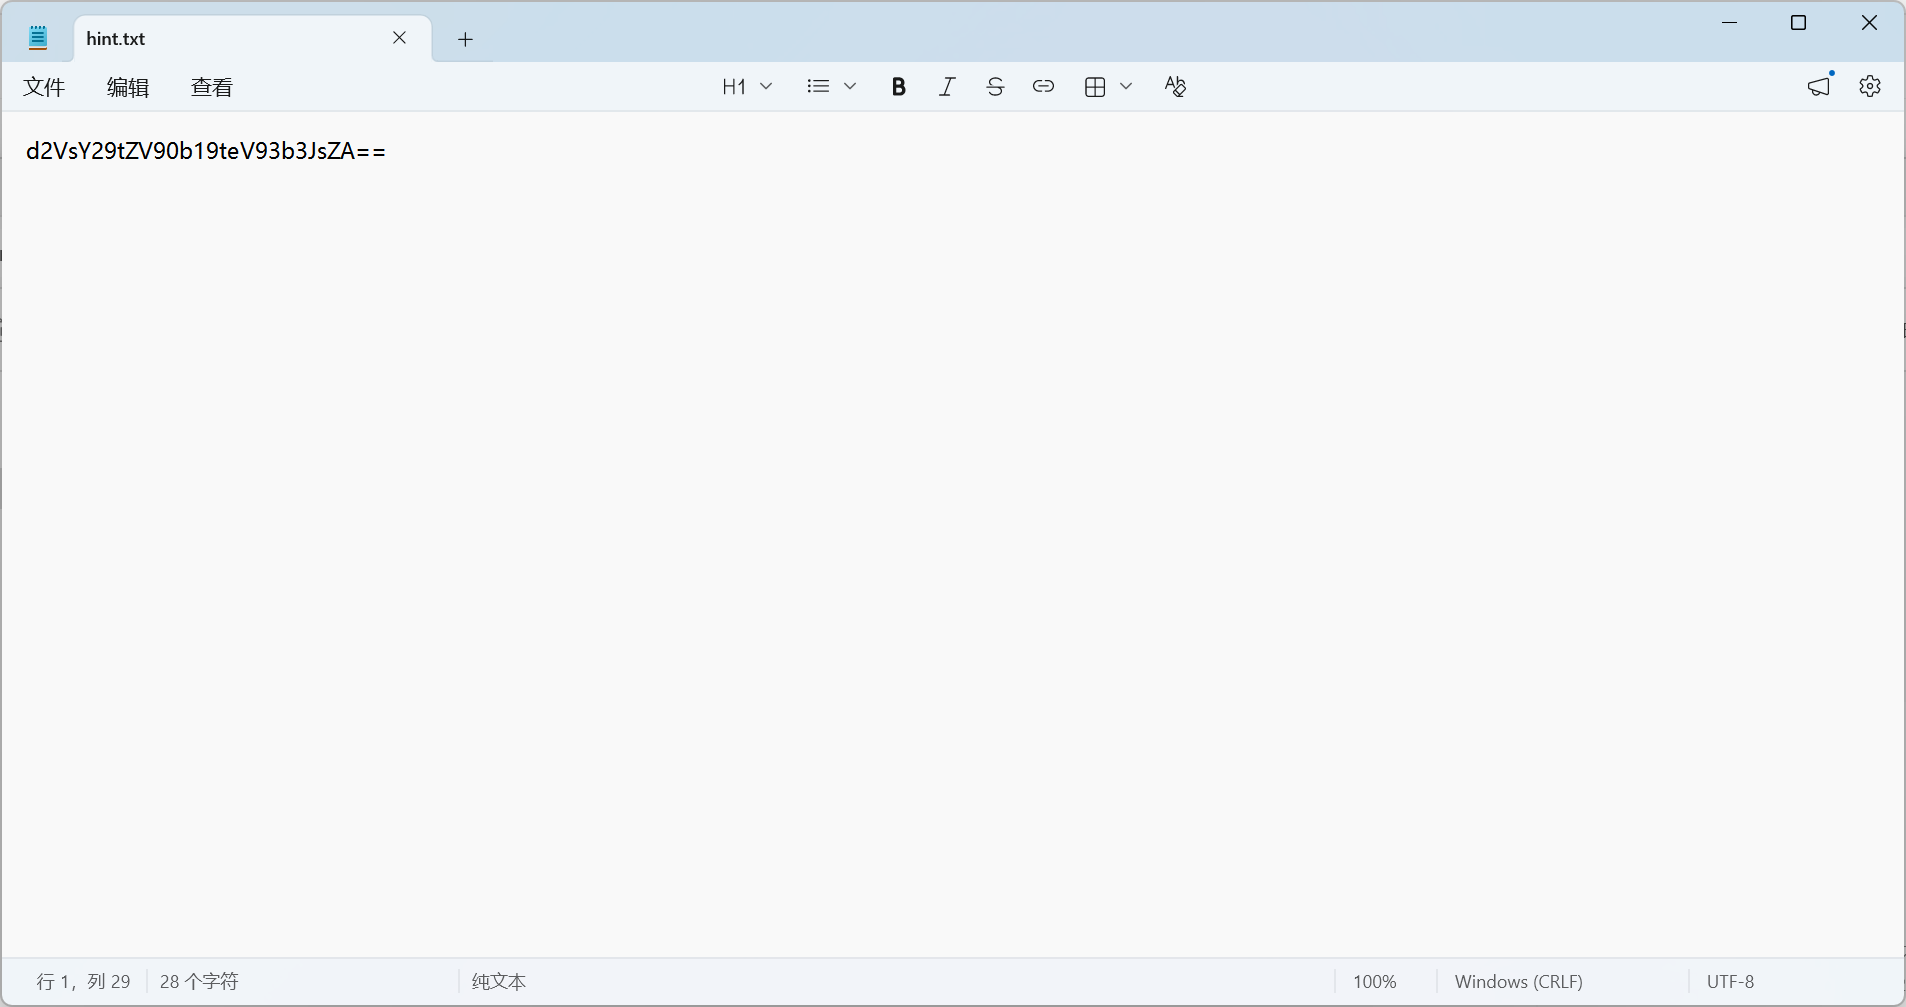
\includegraphics[width=0.95\textwidth]{6.2.png}
    \caption{hint.txt中的Base64密文}
\end{figure}
\begin{figure}[H]
    \centering
    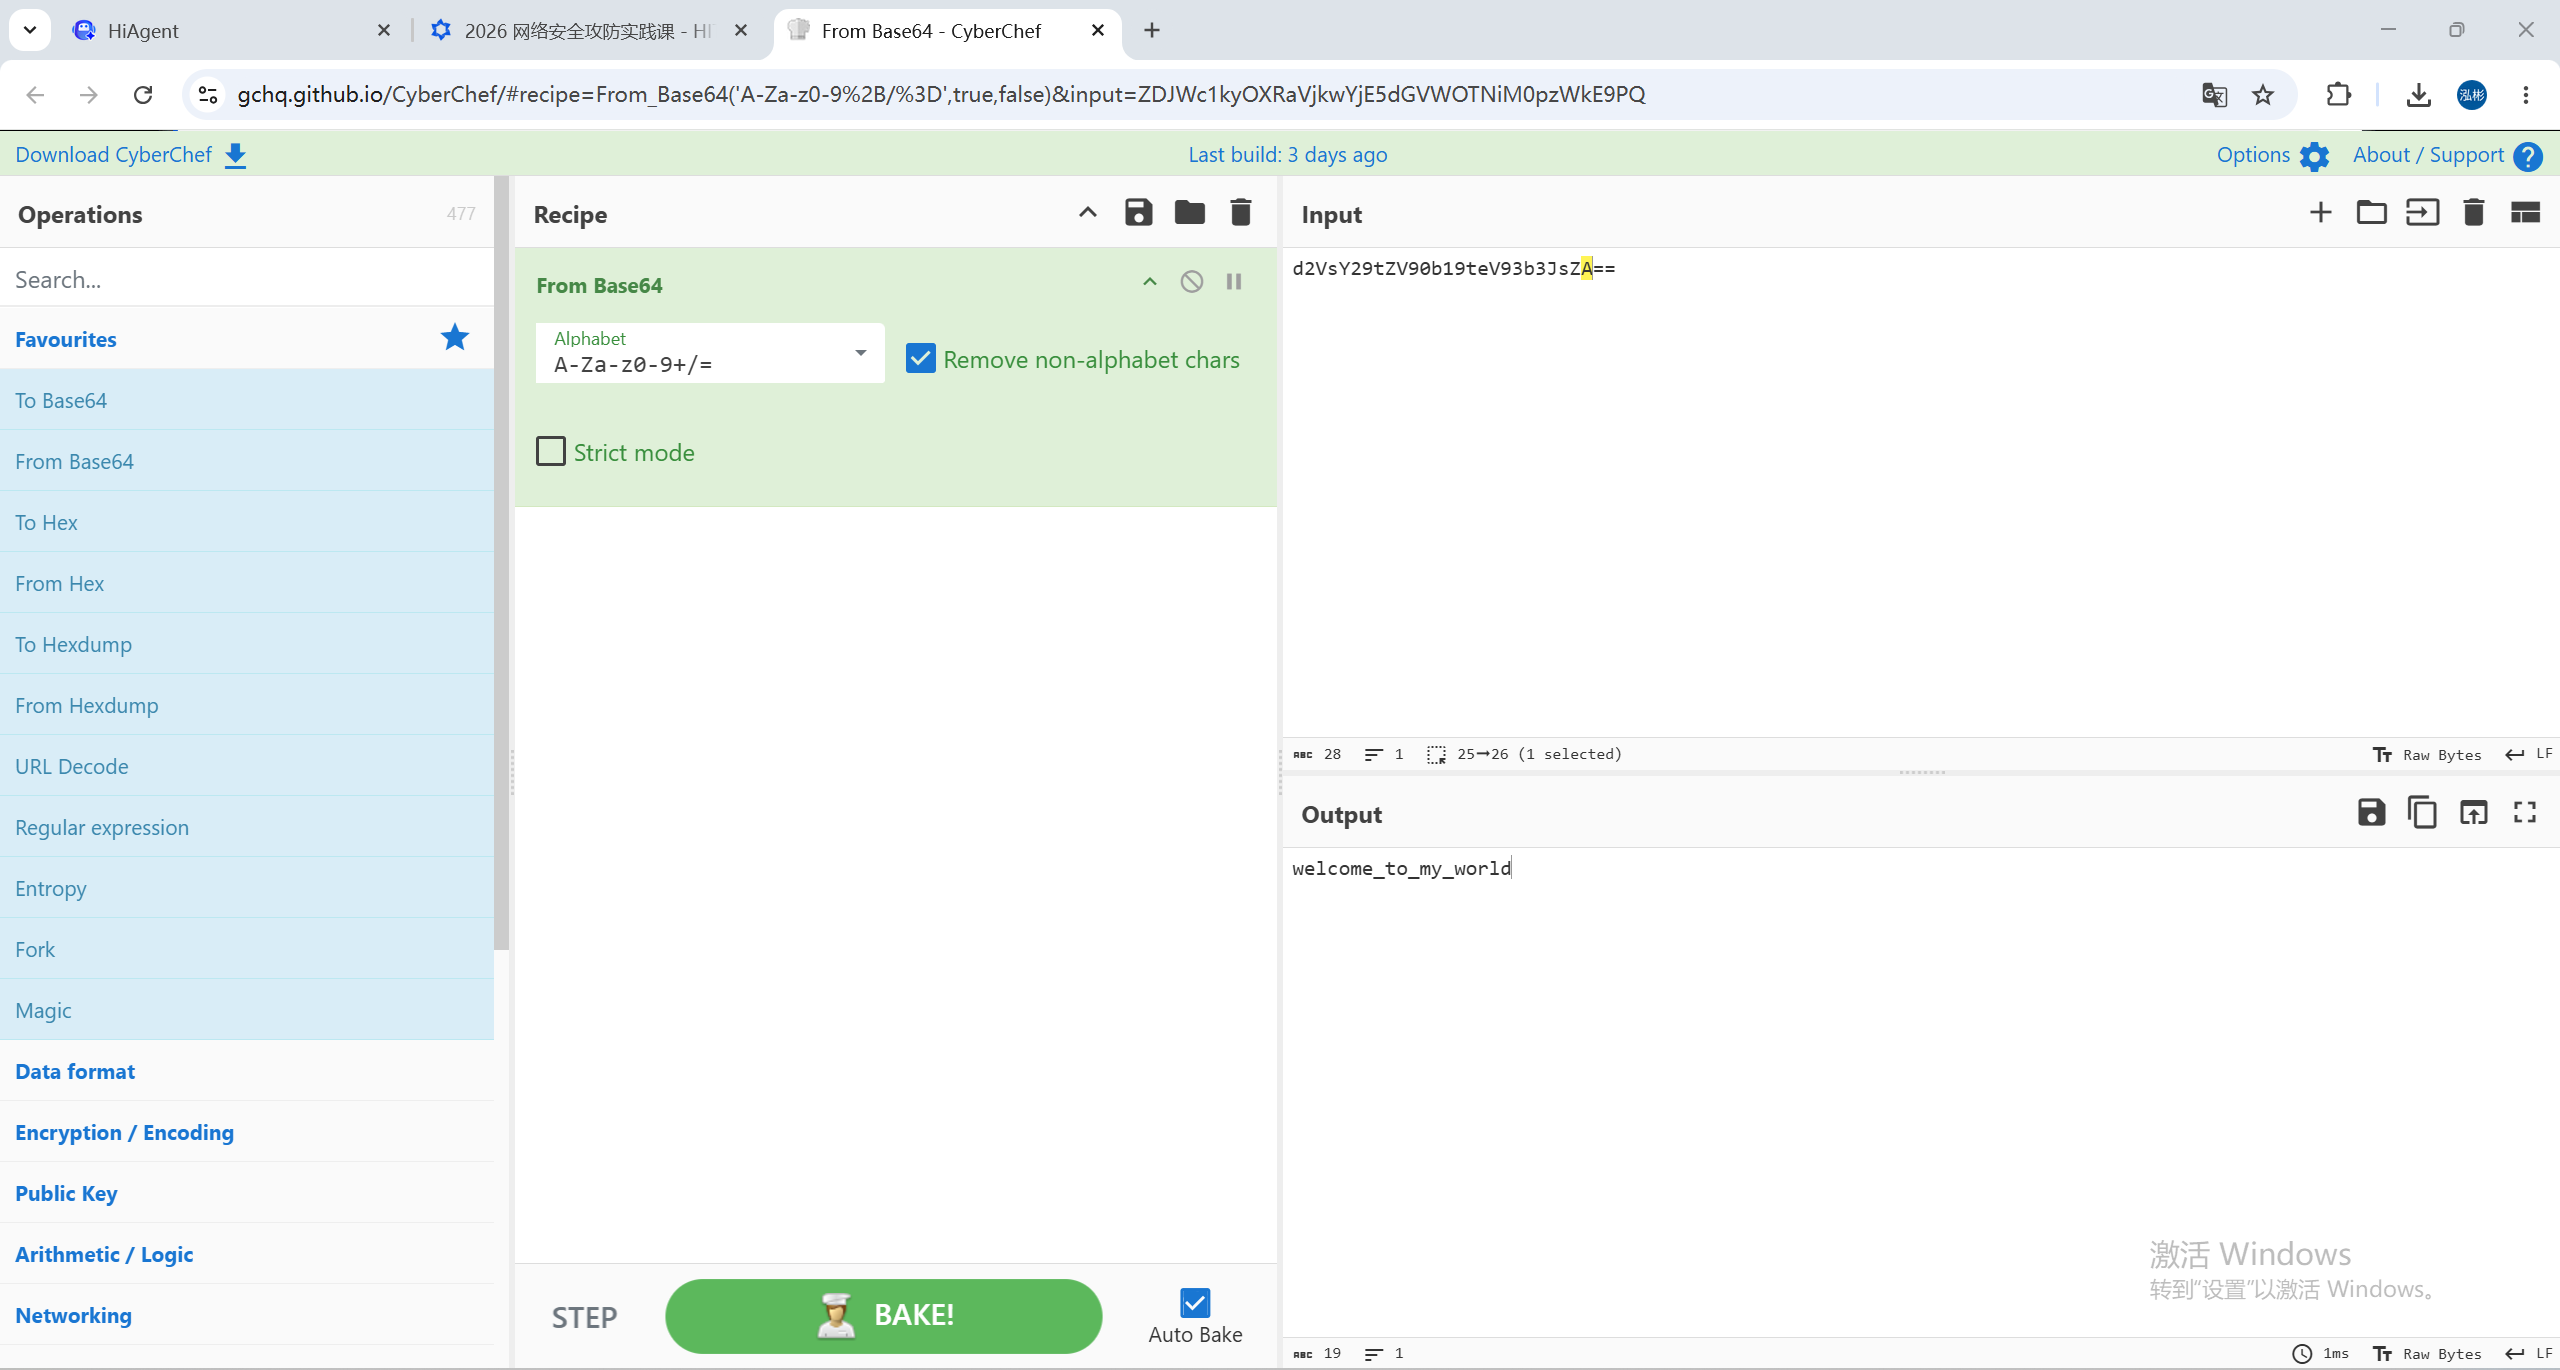
\includegraphics[width=0.95\textwidth]{6.3.png}
    \caption{CyberChef Base64解码得到隐写密码}
\end{figure}
\begin{figure}[H]
    \centering
    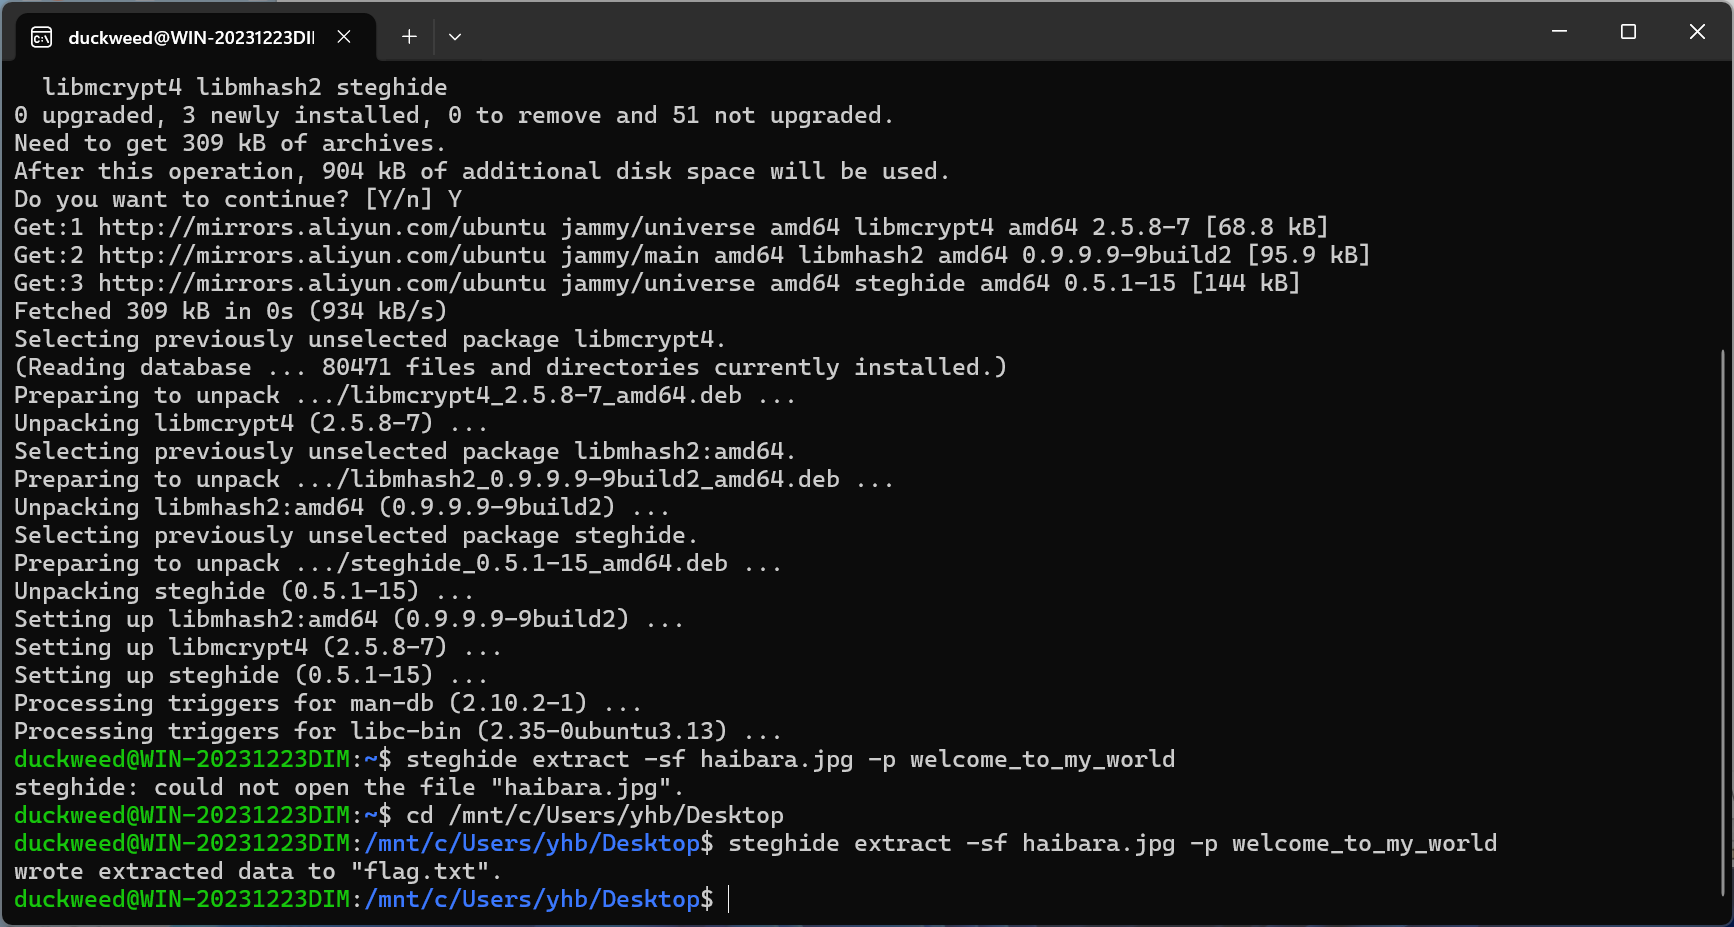
\includegraphics[width=0.95\textwidth]{6.4.png}
    \caption{WSL中使用steghide提取隐写内容}
\end{figure}
\begin{figure}[H]
    \centering
    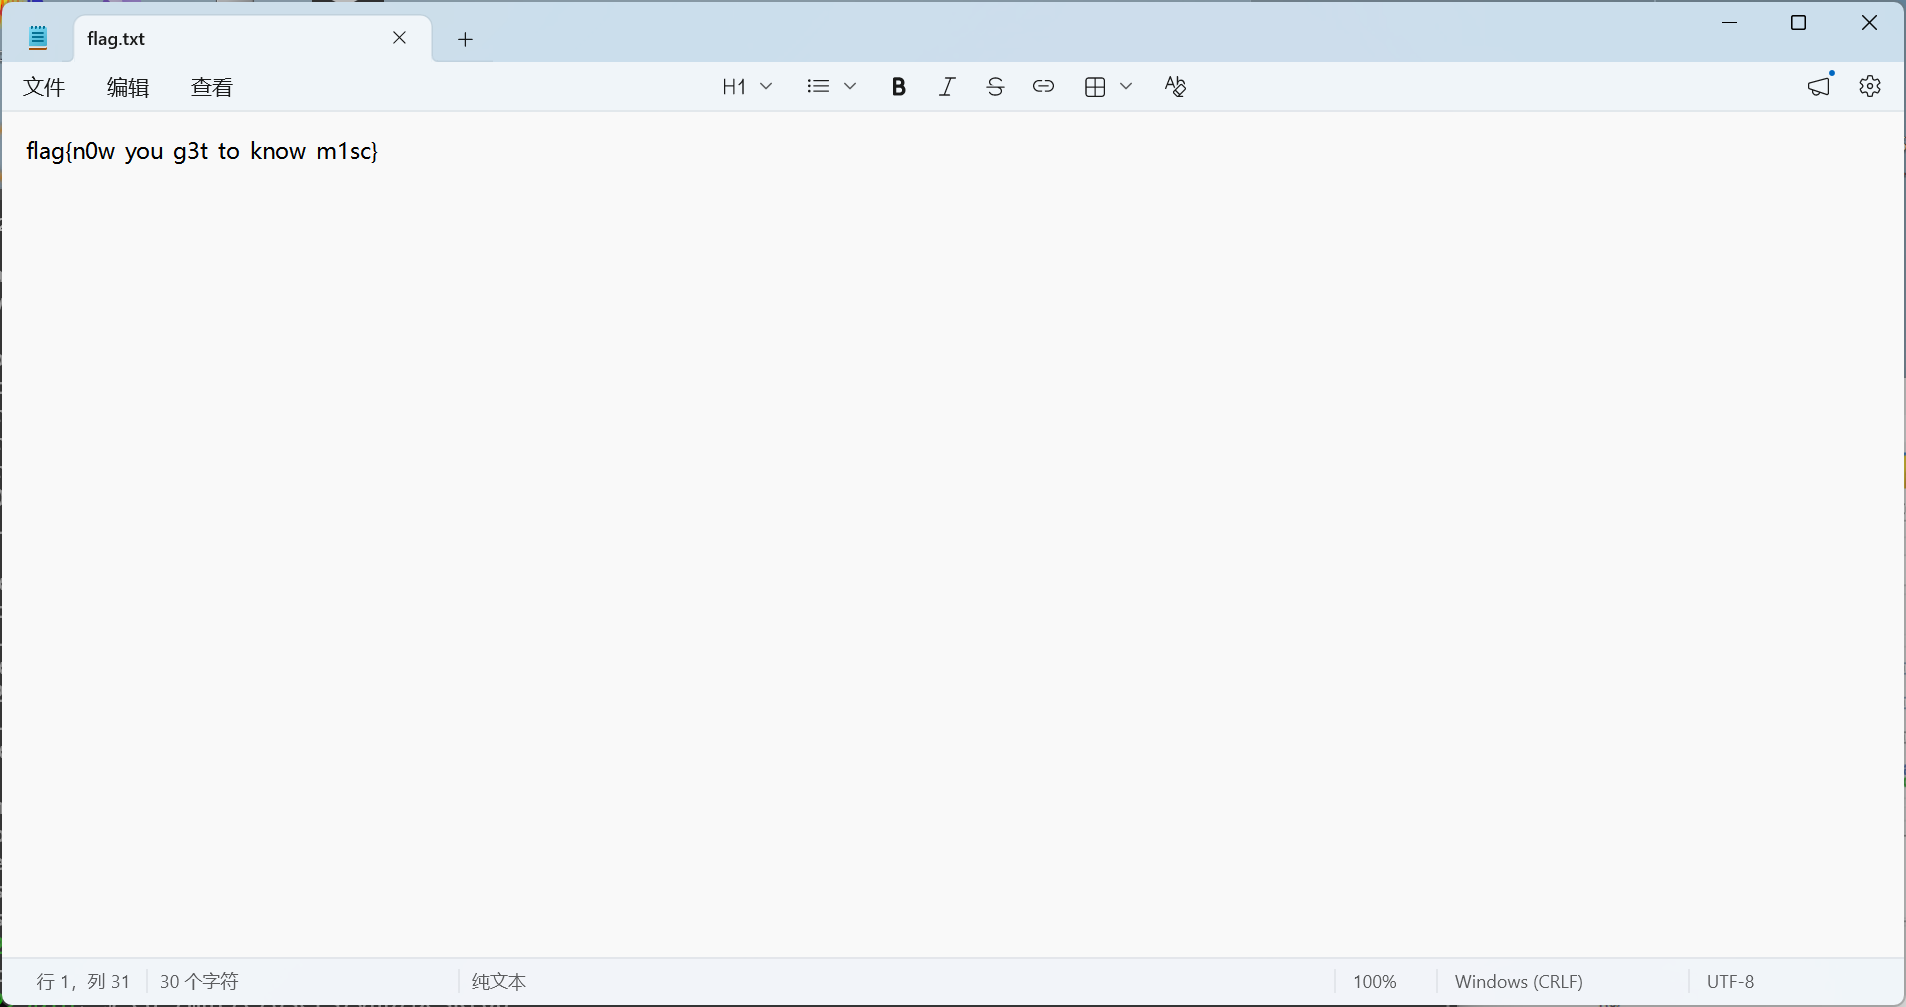
\includegraphics[width=0.95\textwidth]{6.5.png}
    \caption{提取得到的flag.txt}
\end{figure}

\subsection{最终Flag}
\begin{center}
    \Large flag\{n0w you g3t to know m1sc\}
\end{center}

\newpage

% --------------------- 题目7：ZIP 伪加密 + 佛曰解密
\section{题目7：ZIP 伪加密与佛曰解码}
\subsection{解题步骤}
\begin{enumerate}
    \item 使用 010 Editor 打开 ZIP 文件，修改加密标志位为 00，解除伪加密。
    \item 解压得到加密文本，判断为佛曰加密。
    \item 使用佛曰解密工具解码得到最终 flag。
\end{enumerate}

\begin{figure}[H]
    \centering
    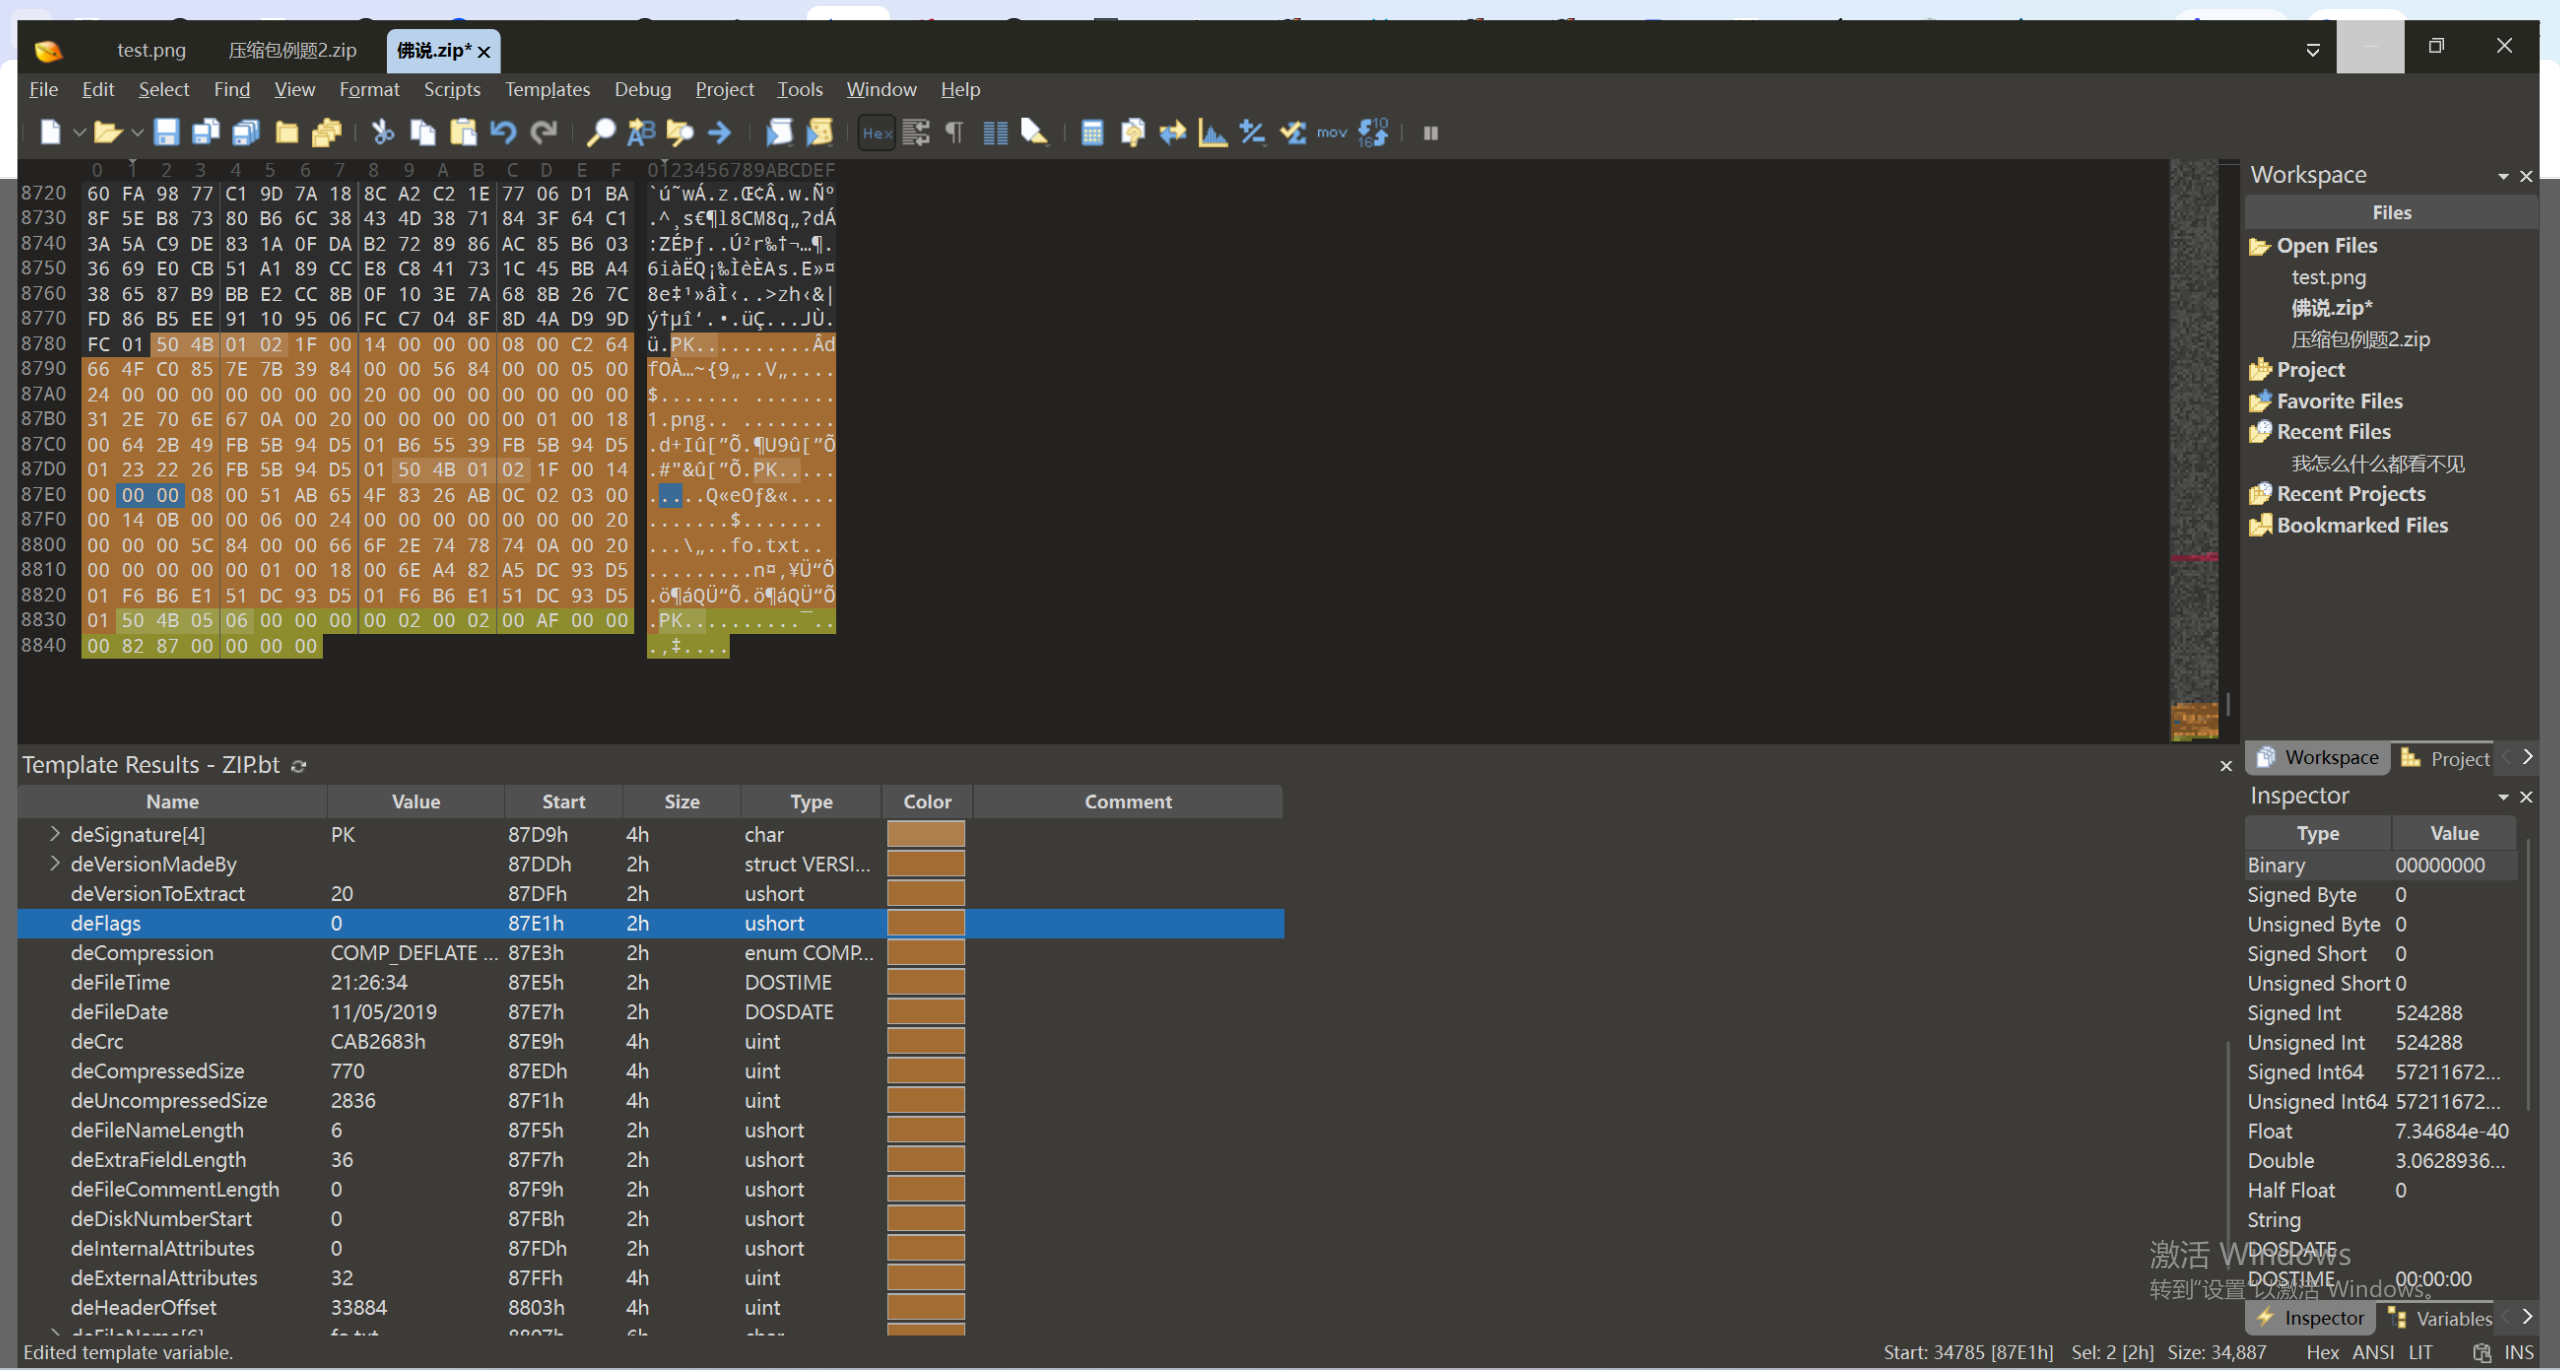
\includegraphics[width=0.95\textwidth]{7.1.png}
    \caption{ZIP 伪加密修复}
\end{figure}
\begin{figure}[H]
    \centering
    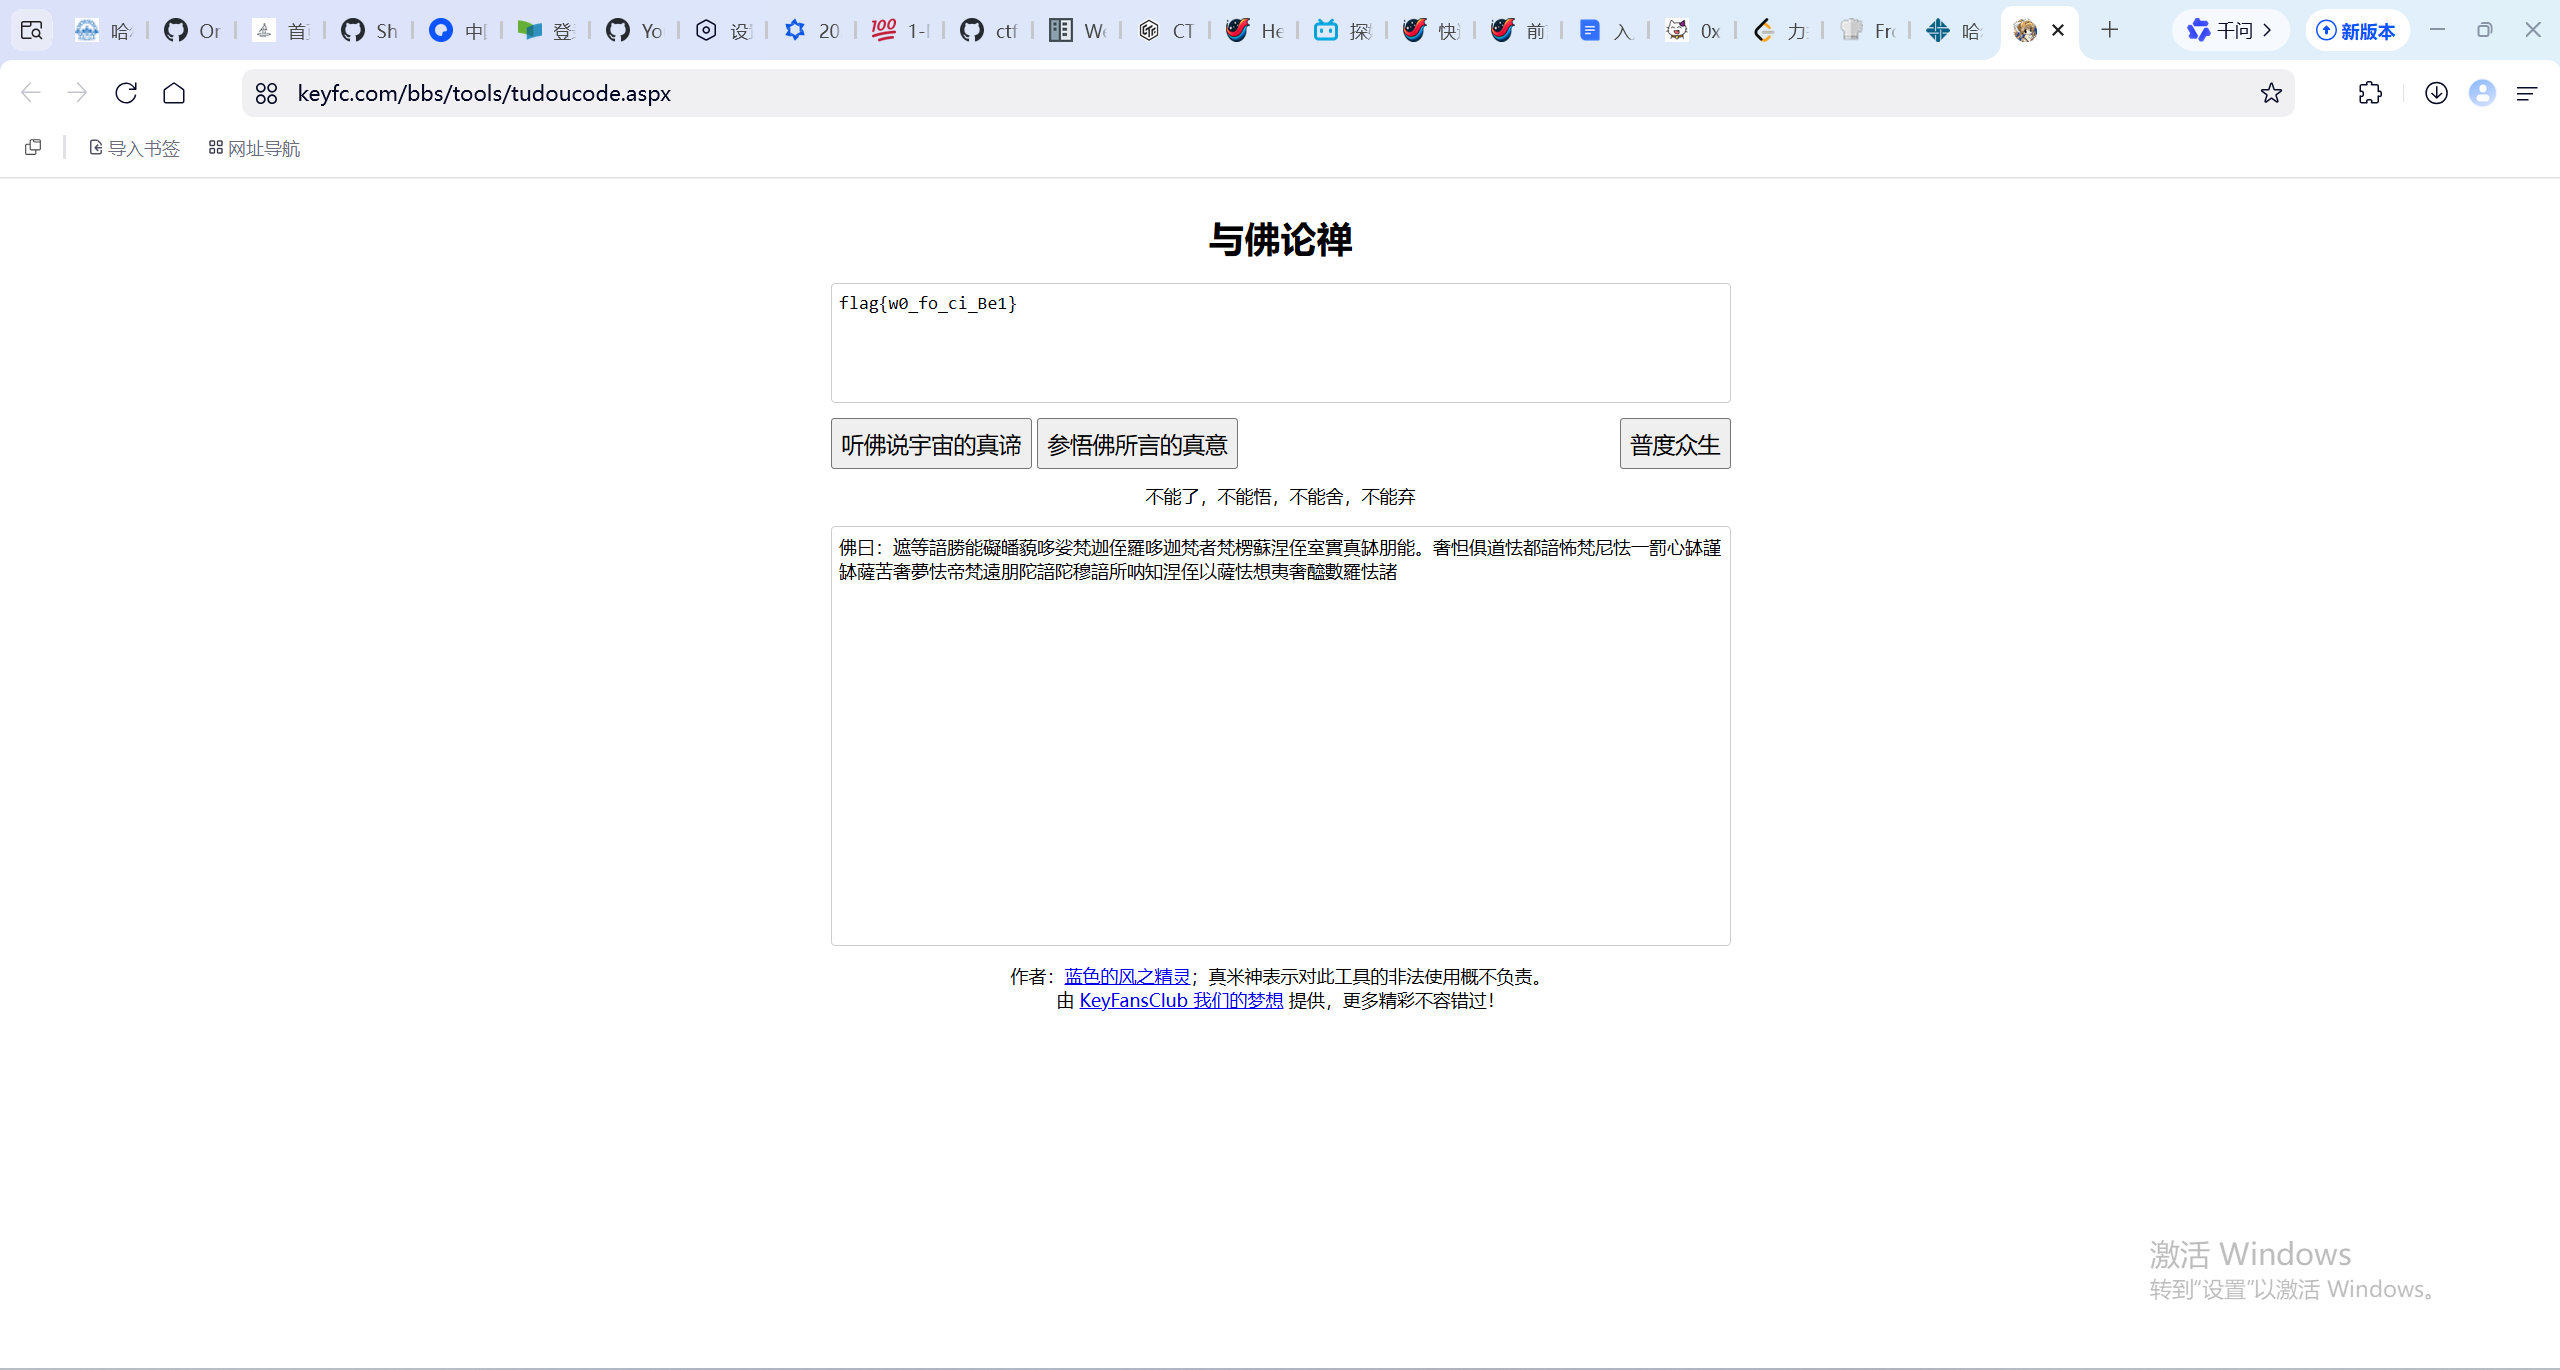
\includegraphics[width=0.95\textwidth]{7.2.png}
    \caption{佛曰加密解密}
\end{figure}

\subsection{最终Flag}
\begin{center}
    \Large flag\{w\_fo\_ci\_Be1\}
\end{center}

\newpage

% --------------------- 题目8：流量分析 PCAP
\section{题目8：流量分析与文件提取}
\subsection{解题步骤}
\begin{enumerate}
    \item 从流量包中提取出疑似文件，修改后缀名为 RAR 并解压。
    \item 使用 Wireshark 打开流量包，追踪 TCP 数据流。
    \item 从数据流中提取关键信息，得到 flag。
\end{enumerate}

\begin{figure}[H]
    \centering
    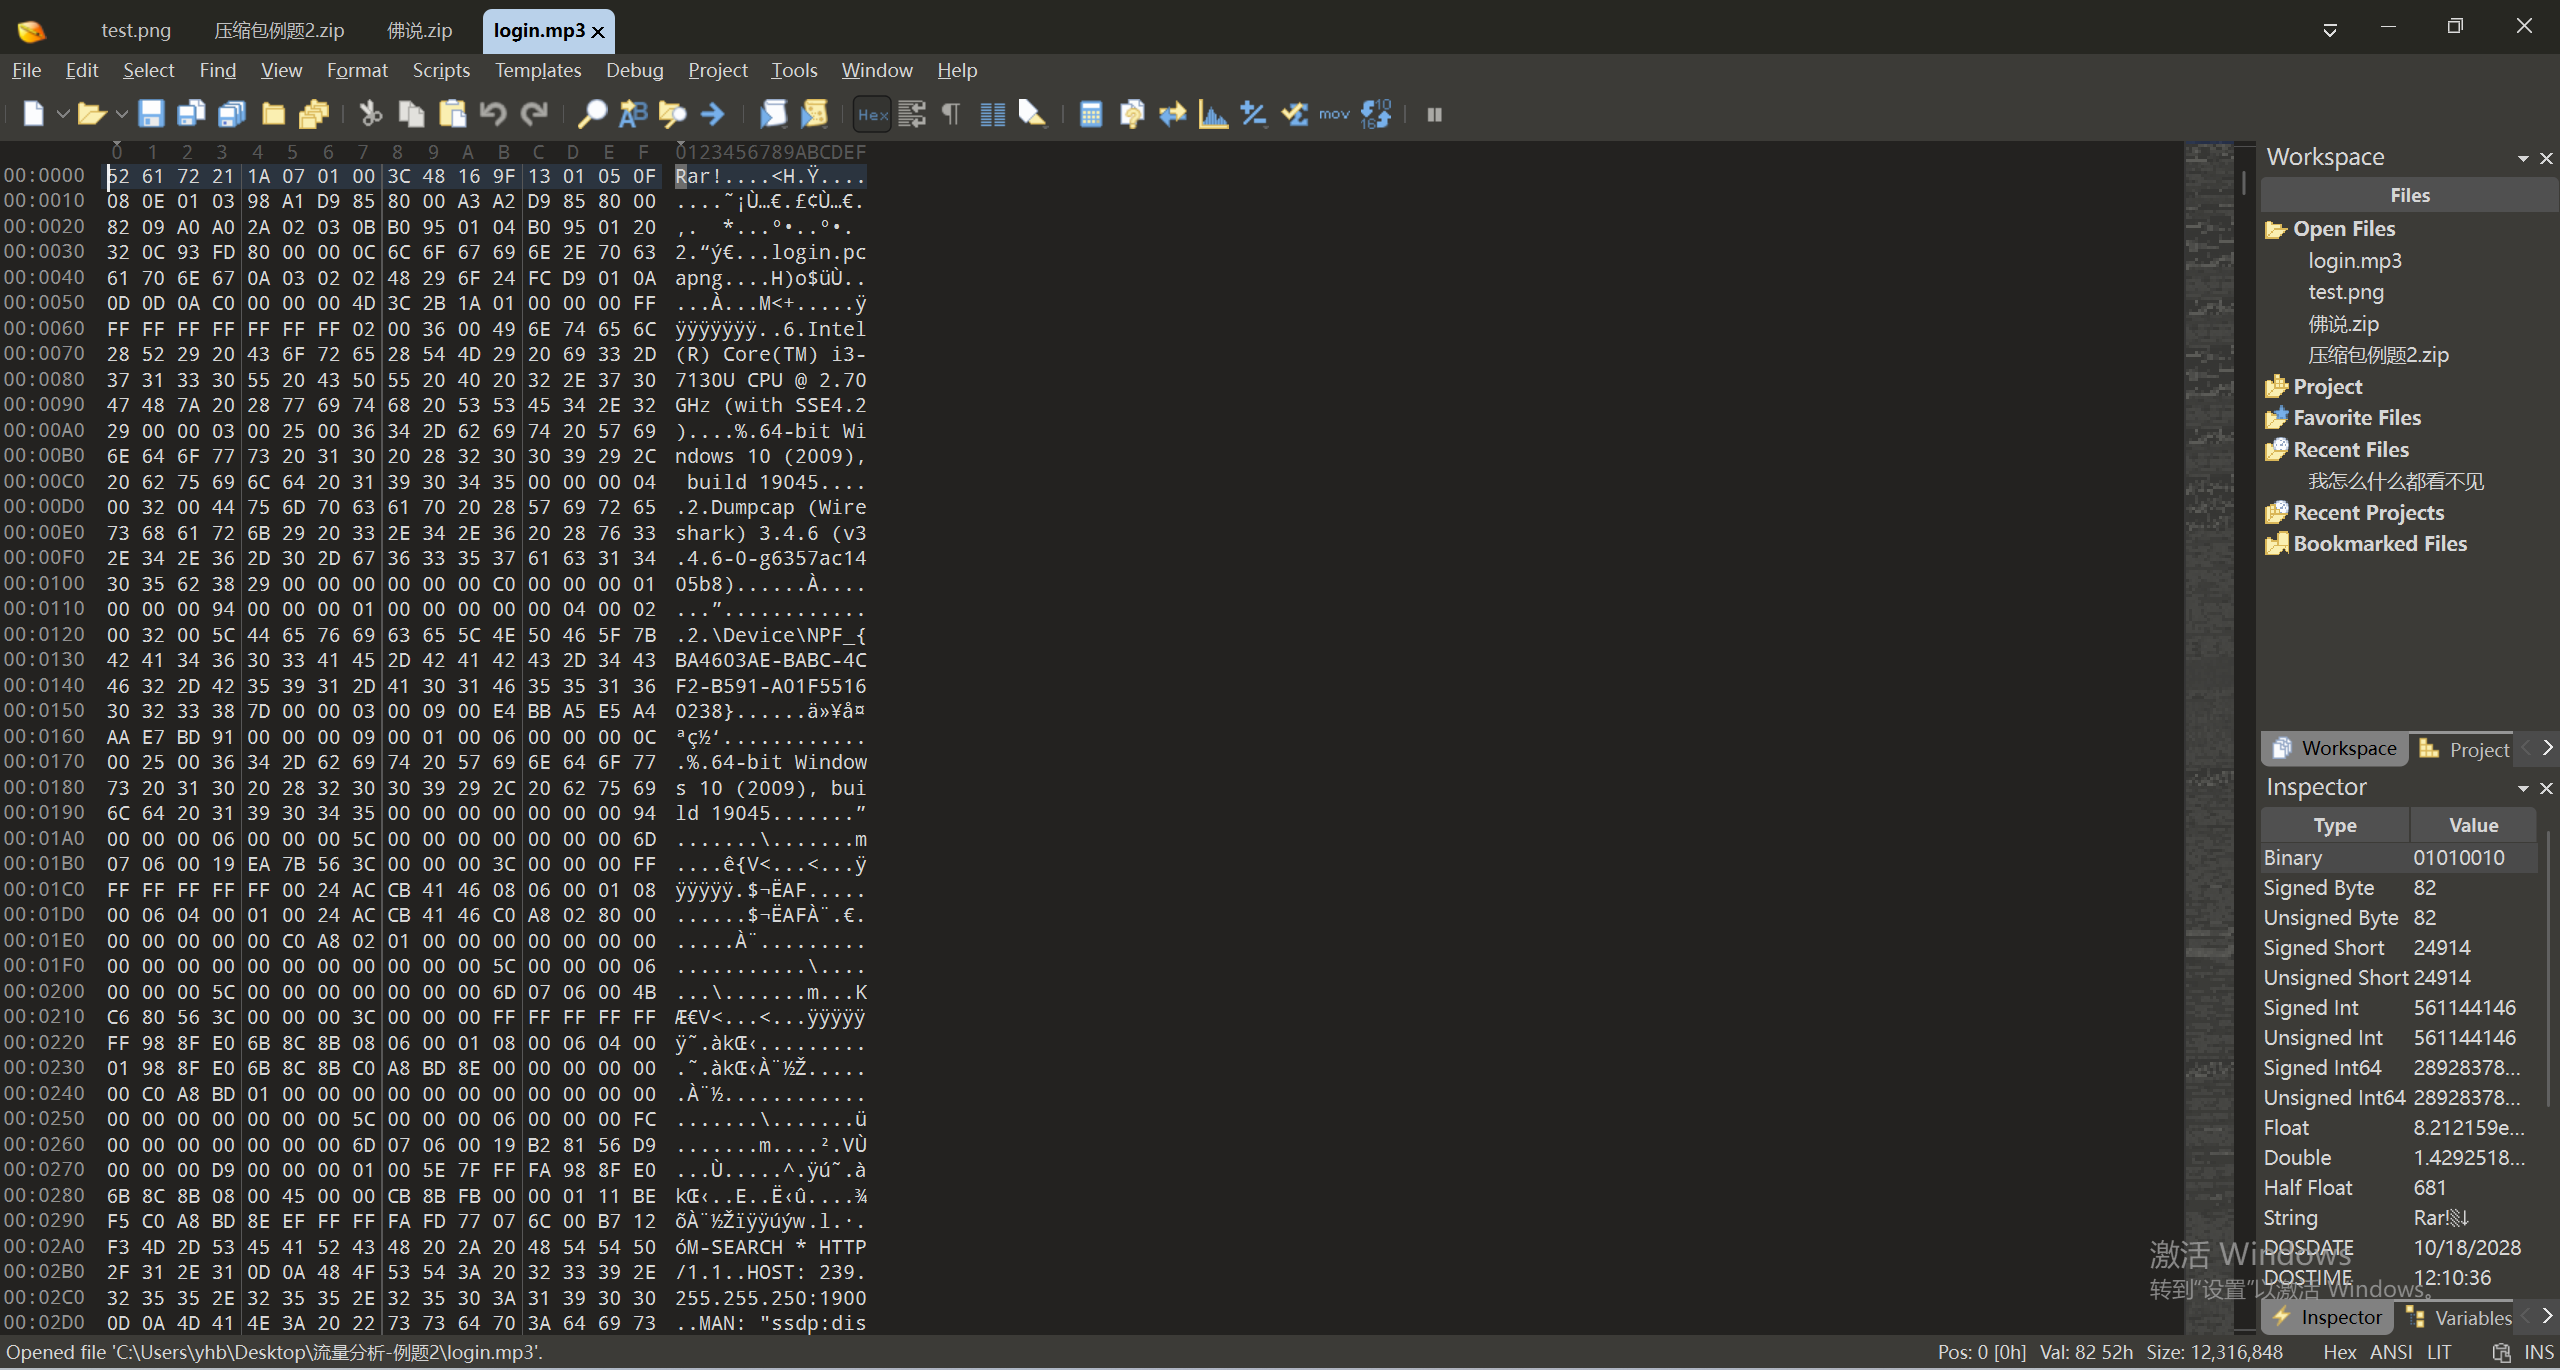
\includegraphics[width=0.95\textwidth]{8.1.png}
    \caption{文件头识别与格式修改}
\end{figure}
\begin{figure}[H]
    \centering
    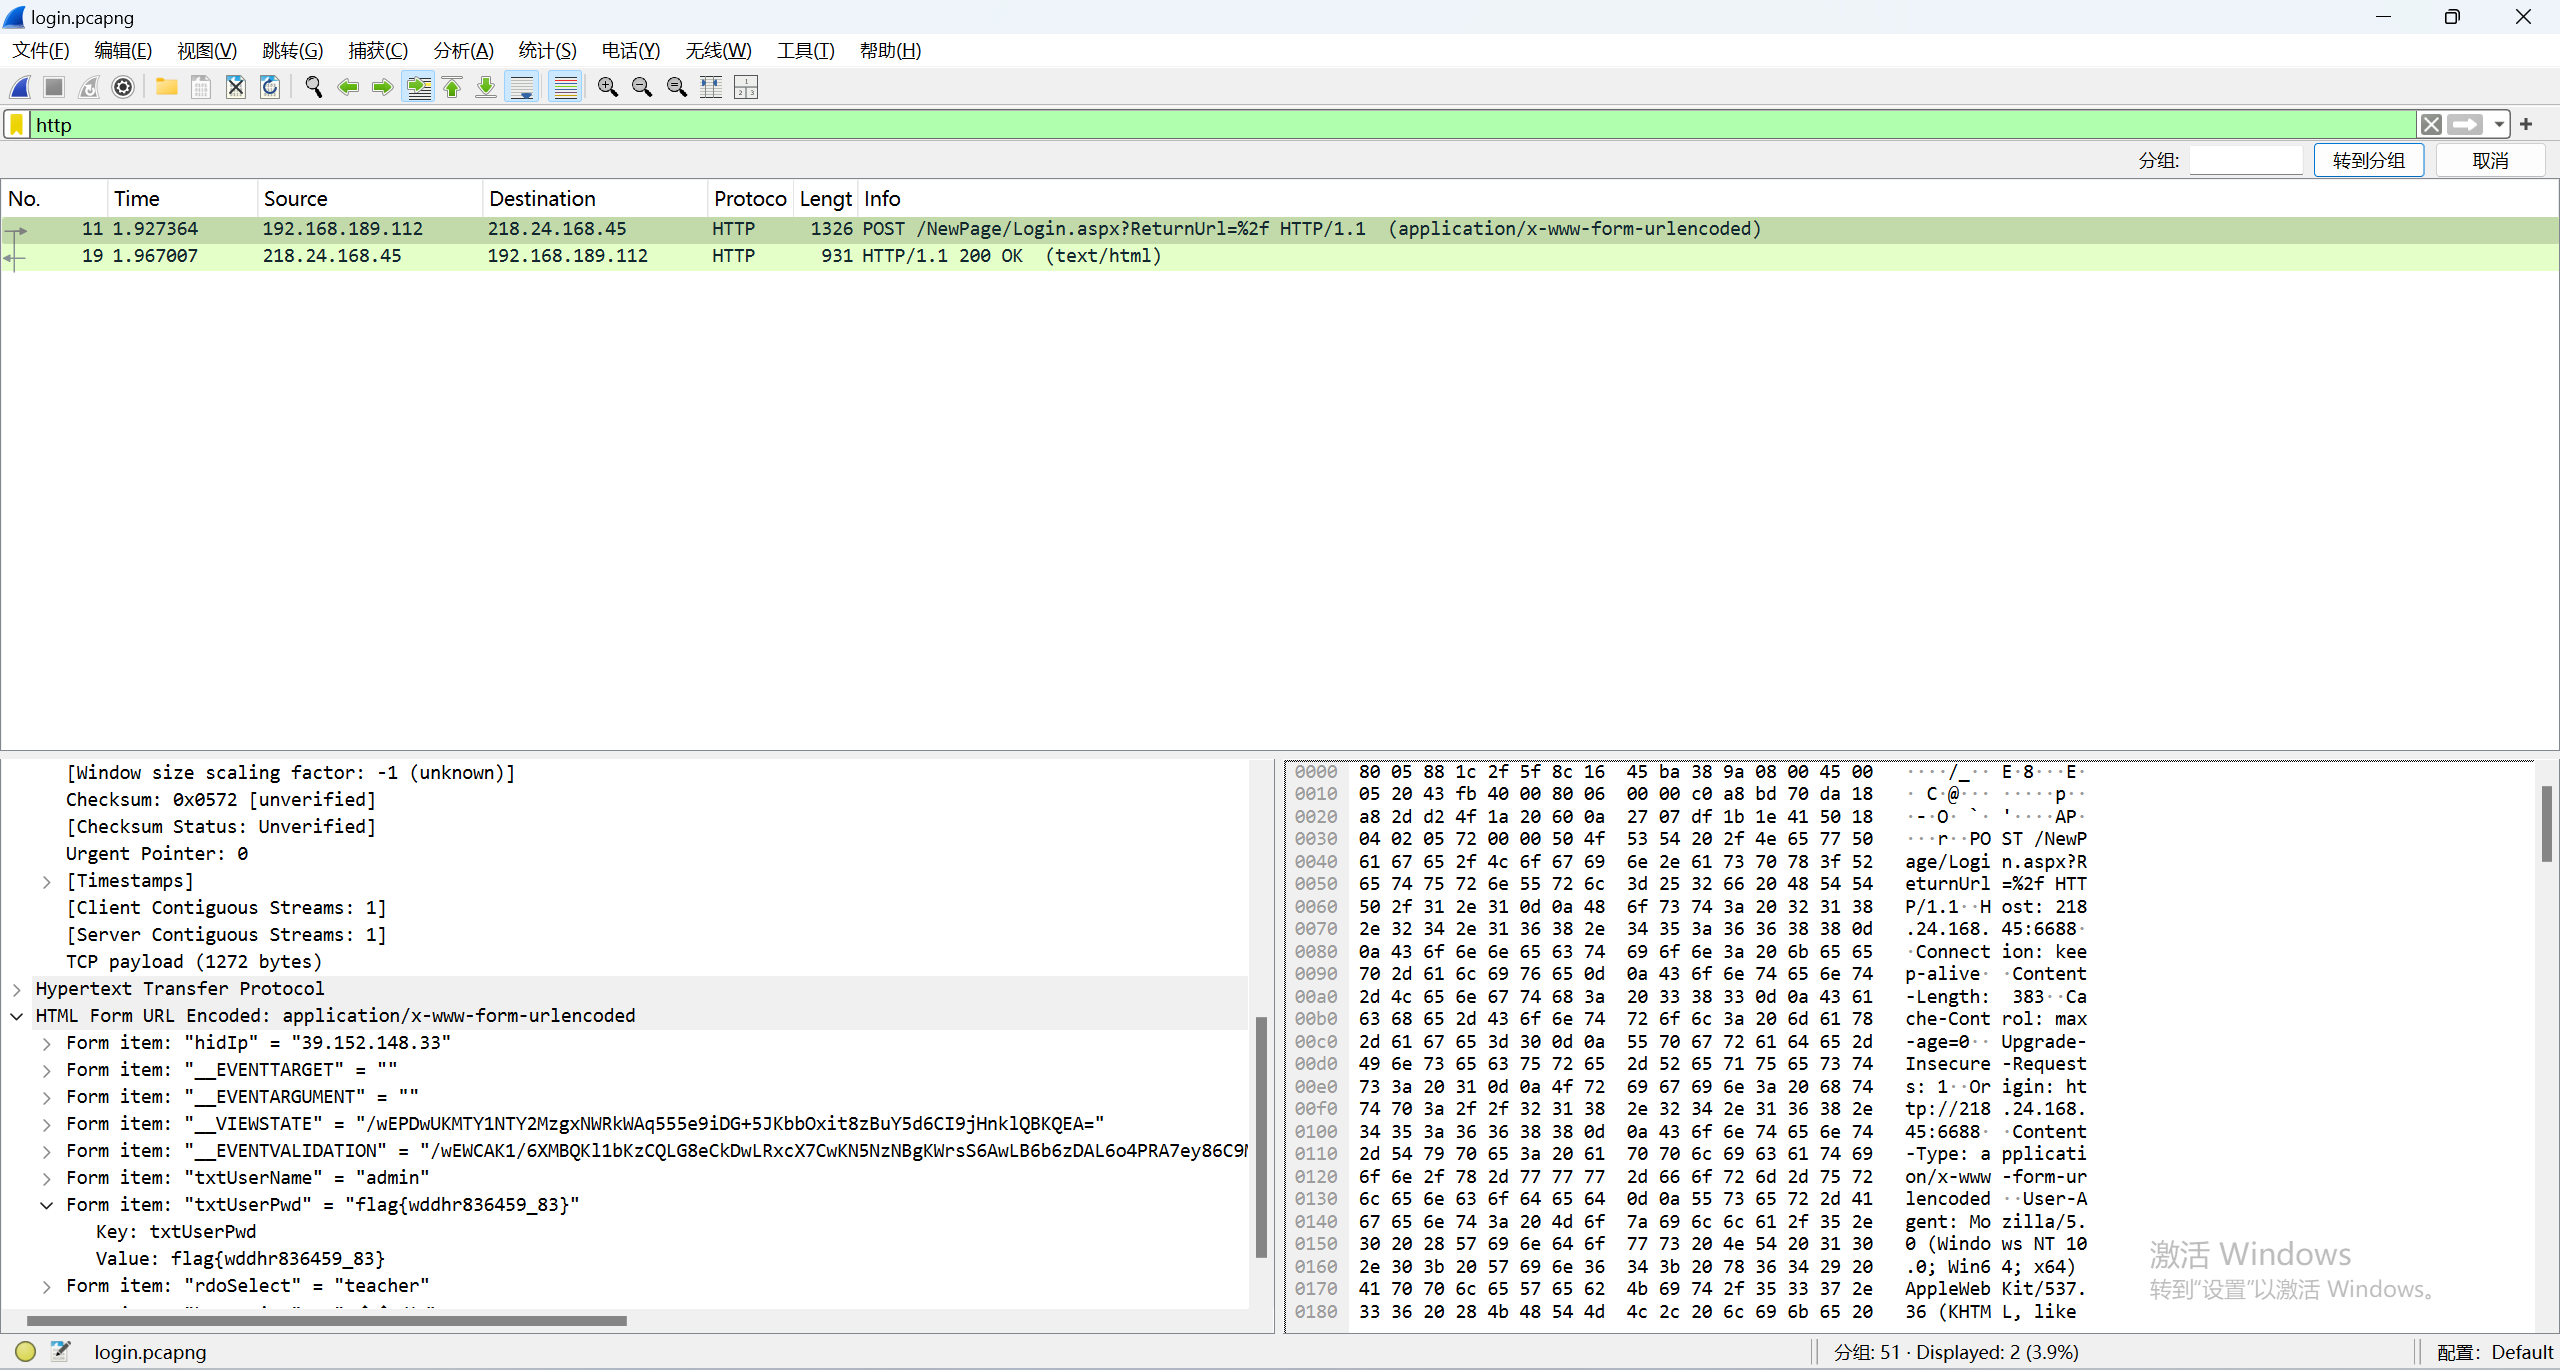
\includegraphics[width=0.95\textwidth]{8.2.png}
    \caption{Wireshark TCP 流追踪}
\end{figure}

\subsection{最终Flag}
\begin{center}
    \Large flag\{wddhr836459\_83\}
\end{center}

\newpage

% --------------------- 题目10
\section{题目10：PyJail 沙箱绕过}
\subsection{解题步骤}
\begin{enumerate}
    \item 分析 Python 沙箱限制，寻找可用内置函数与绕过方法。
    \item 构造绕过语句读取 flag 文件。
    \item 执行语句得到最终 flag。
\end{enumerate}

\subsection{最终Flag}
\begin{center}
    \Large flag\{************************\}
\end{center}

\end{document}